\documentclass[11pt]{article}

\usepackage{amsmath}
\usepackage{float}
\usepackage{parskip}
\usepackage{amsfonts}
\usepackage{geometry}
\usepackage{amsthm}

\usepackage{pgfplots}

\pgfplotsset{width=10cm,compat=1.9}
\usepgfplotslibrary{external}
\tikzexternalize

% commands
\newcommand{\set}[1]{\{#1\}}
\newcommand{\given}{\, | \,}
\newcommand{\real}{\mathbb{R}}
\newcommand{\nat}{\mathbb{N}}
\newcommand{\inv}[1]{{#1}^{-1}}
\newcommand{\rank}[1]{\text{rank}\, #1}

\usepackage{tcolorbox}
\usepackage{amssymb}
\tcbuselibrary{theorems}
\newtcbtheorem
[auto counter, number within = section]% init options
{theorems}% name
{Theorem}% title
{%
	colback=green!5,
	colframe=green!60!black,
	fonttitle=\bfseries,
	sharp corners
}% options
{def}% prefix

\newtcbtheorem
[auto counter, number within = section]% init options
{lemmas}% name
{Lemma}% title
{%
	colback=red!5,
	colframe=red!60!black,
	fonttitle=\bfseries,
	sharp corners
}% options
{def}% prefix

\newtcbtheorem
[auto counter, number within = section]% init options
{algor}% name
{Algorithm}% title
{%
	colback=green!5,
	colframe=green!70!black,
	fonttitle=\bfseries,
	sharp corners
}% options
{def}% prefix

\newtcbtheorem
[auto counter, number within = section]% init options
{iden}% name
{Identity}% title
{%
	colback=yellow!5,
	colframe=yellow!70!black,
	fonttitle=\bfseries,
	sharp corners
}% options
{def}% prefix

\newtcbtheorem
[auto counter, number within = section]% init options
{defn}% name
{Definition}% title
{%
	colback=red!5,
	colframe=red!70!black,
	fonttitle=\bfseries,
	sharp corners
}% options
{def}% prefix


\newtheorem{theorem}{Theorem}[section]
\newtheorem{corollary}{Corollary}[theorem]
\newtheorem{lemma}[theorem]{Lemma}

\DeclareMathOperator{\spann}{span}
\newcommand{\coord}[2]{[#1]_{#2}}

\usepackage{mathtools}
\DeclarePairedDelimiter\ceil{\lceil}{\rceil}
\DeclarePairedDelimiter\floor{\lfloor}{\rfloor}


\DeclareMathOperator{\rowspace}{rowspace}
\DeclareMathOperator{\colspace}{colspace}
\DeclareMathOperator{\im}{im}


\title{Calculus Advanced}
\author{T QI}
\date{}

\begin{document}

\maketitle
\newpage

\tableofcontents
\newpage



\section{Numbers, Intervals, Inequalities}

\subsection{Induction}
Define the natural numbers to be the counting numbers without zero
\begin{align*}
	\mathbb{N} &= \set{1,2,3,\dots}\\
\end{align*}

Proofs using induction are used to prove statements of the form that $\forall n \in \mathbb{N}$, the statement $p(n)$ holds. It suffices to prove that $p(1)$ holds, and that if $p(k)$ for $k \in \mathbb{N}$ holds, $p(k+1)$ will also hold.

\begin{proof}
	To show that the upper bound holds for $\forall a \geq 1, \forall n \in \mathbb{N}$
	\[
		\sum_{i=1}^{n} i^2 \leq a n^3
	\]

	Consider the induction on $n$. The base case is
	\[
		\sum_{i=1}^1 i^2 = 1 \leq a 1^2
	\]
	which is true for all $a \geq 1$.

	Now assume that the case holds for $n = k$, where
	\[
		\sum_{i=1}^k i^2 \leq a k^3
	\]
	Consider the case $n = k+1$. Where
	\begin{align*}
		\sum_{i=1}^k i^2 + (k+1)^2 &\leq a k^3 + (k+1)^2\\
		ak^3 + (k+1) &= ak^3 + k^2 + 2k + 1\\
		&\leq ak^3 + 3a k^2 + 3a k + a\\
		&= a (k+1)^3\\
		\sum_{i=1}^{k+1} i^2 &\leq a (k+1)^3
	\end{align*}

	Hence the case $n=k+1$ also holds.

	Therefore by the principle of mathematical induction, the upperbound statement holds for all natural numbers $\forall n \in \mathbb{N}$.
\end{proof}
% write the proof that 1^2+2^2+3^2 + ... <= 75 n^3 using induction


\subsection{Number Sets}
Other sets of numbers are
\begin{align*}
	\mathbb{Z} &= \set{\dots, -2, -1, 0, 1, 2, \dots}\\
	\mathbb{Q} &= \set{ \frac{m}{n} \given m, n \in \mathbb{Z}, n \neq 0}
\end{align*}

Note that
\[
	\mathbb{Q} \not \equiv (\mathbb{Z} \times \mathbb{Z} \setminus \set{0})
\]
because fractions can be simplified.

Types of proofs are: induction, contradiction, and contrapositive.

We can prove by contradiction that $\sqrt{2}$ is irrational, ie, $\sqrt{2} \notin \mathbb{Q}$.

\subsection{Inequalities}

The theorems relating inequalities are
\[
	a < b \quad \text{iff} \quad b > a
\]

\begin{iden}{Inequality Trichotomy}{}
	For all real numbers $a$ and $b$, only one of the following assertions hold.
	\begin{align*}
		a &< b\\
		a &> b\\
		a &= b
	\end{align*}
\end{iden}

\begin{iden}{Inequality Ordering}{}
	For any numbers $a$, $b$, and $c$
	\[
		a < b \land b < c \implies a < c
	\]
\end{iden}

\begin{iden}{Inequality Closures}{}
	For any numbers $a$, $b$, and $c$
	\[
		a < b \implies a + c < b + c
	\]
	this is the concept of translational invariance.

	and if $c > 0$
	\[
		a < b \implies ca < cb
	\]
	which denotes positive scalar invariance.
\end{iden}

All the other inequality theorems can be deduced from these three axioms.

\subsection{Intervals}
Definition of intervals like $(a, b)$, $(a, b]$, $[a, b]$.

The absolute value function on the real numbers is defined to be
\[
	\forall x \in \mathbb{R}, |x| = \begin{cases}
		x & \text{if}\quad x\geq 0\\
		-x & \text{if}\quad x < 0
	\end{cases}
\]

\begin{iden}{Absolute Value Identities}{}
For any real $x$:
\begin{align*}
	x^2 &= |x|^2\\
	ab &\leq |ab| = |a| |b|\\
	x^2\leq y^2 &\implies |x| \leq |y|
\end{align*}
\end{iden}

\begin{theorems}{Triangle Inequality}{}
The triangle inequality states that for $a, b \in \mathbb{R}$
\[
	|a + b| \leq |a| + |b|
\]
also
\[
	|a - b| \geq |a| - |b|
\]
\end{theorems}


\subsection{Euclidean Space}
Define the space $\mathbb{R}^n$ for $n \in \mathbb{N}$ to be an n-dimensional space with points having coordinates that are n-ordered tuples.

We can treat coordinates as vectors, with the operations of: vector addition and scalar multiplication.

\begin{defn}{Length and Dot product}{}
Define the length of a vector by the dot product, where
\[
	|x| = \sqrt{x \cdot x}
\]
where
\[
	a \cdot b = \sum_i a_i b_i
\]

Notice that
\[
    |x|^2 = x \cdot x
\]
\end{defn}

Two vectors are orthogonal iff $a \cdot b = 0$.

\begin{theorems}{Vector triangle inequality}{}
The triangle inequality also holds for vectors
\[
	|a + b| \leq |a| + |b|
\]
\end{theorems}
The proof relies on the Cauchy-Schwartz inequality, which is, for any vector $a$ and $b$,
\[
	|a\cdot b| \leq |a| |b|
\]
with equality when $a$ and $b$ are parallel.
\begin{proof}
    To prove the Cauchy-Schwartz with dot products, we consider the function
    \[
    f(t) = |a - tb|^2 = |a|^2 - 2t a\cdot b + t^2 |b|^2
    \]
    specifically at its minima, at $t = a\cdot b / |b|^2$. And notice that $f(t) \geq 0$ and thus the substituted RHS will also be positive, and hence retrieving the inequality after rebalancing.

    To show the triangle inequality, we expand out $|x+y|^2$ and substitute the CS inequality to get the triangle inequality with squares. By taking square roots, we can prove the triangle inequality.
\end{proof}

\begin{defn}{Vector distance}{}
Define the distance between point $a$ and point $b$ as $|a - b| = | b - a |$.
\end{defn}


\newpage
\section{Functions and Graphs}
We want to explore functions of the form
\[
	f \colon \mathbb{R}^2 \to \mathbb{R}
\]

Define
\[
	\mathbb{R}^2 = \mathbb{R} \times \mathbb{R}
\]

We can treat points in $\mathbb{R}^2$ as vectors --- we can add vectors, and multiply vectors with scalars.

Define the analog of the absolute value in vectors $\mathbb{R}^2$ as
\[
	x = (a,b) \in \mathbb{R}^2, ||x|| = \sqrt{a^2+b^2}
\]

The triangle inequality in $\mathbb{R}^2$ is such that for $x, y \in \mathbb{R}^2$,
\[
	||x+y|| \leq ||x|| + |y||
\]

Define the 2D dot product as
\[
	(a,b) \cdot (c,d) = ac + bd
\]

The dot product properties are
\begin{align*}
	||x||^2 &= x \cdot x\\
	||x+y||^2 &= ||x||^2 + 2 (x \cdot y) + ||y||^2\\
	x \cdot y &\leq ||x|| ||y||
\end{align*}
We can prove the triangle inequality theorem (eq 2) by expanding out the square of the lhs and apply Cauchy-Schwarz.

\subsection{Graphs}
A mapping from a domain $A$ to a codomain $B$, where $A$ and $B$ are sets.

The graph of $f \colon A \to B$ where $A \subseteq \mathbb{R}$ is defined to be
\[
	\operatorname{graph}(f) = \set{(x, f(x)) \given x \in A} \subseteq \mathbb{R}^2
\]

For $g \colon A \to B$ where $A \subseteq \mathbb{R}^2$, its graph is
\[
	\operatorname{graph}(g) = \set{(x,y,g(x,y)) \given (x, y) \in A} \subseteq \mathbb{R}^3
\]


In general for a function $f \colon A \to B$ for the domain $A$ and codomain $B$, its graph is
\[
	\operatorname{graph}(f) = \set{ (x, f(x)) \given x \in A} \subseteq A \times B
\]

The combination of function is only defined on their domain intersection.

Function composition only makes sense if the domain matches the other's codomain.

A rational function has the form:
\[
	f(x) = \frac{p(x)}{q(x)}
\]
where $p(x)$ and $q(x)$ are polynomials.

To sketch a graph, note its bounds (maximums and minimums), whether the function approaches or equals its bounds, and roots of the function. We can also consider its value near singularities and infinities to guess its shape.

\subsection{Multivariate functions}

2D polynomials have the form
\[
	p(x,y) = \sum_{i, j} a_{ij} x^i y^j
\]
The degree of each term $a_{ij}$ is $i + j$, and the degree of the polynomial is the maximum degrees of its term.


To visualize real valued 2D functions, we consider its graph --- the graph of such a function forms a surface in $\mathbb{R}^3$. Because it is difficult to sketch a surface, we consider its slices, which are curves that are easier to visualize.

One method is to restrict the domain to a 2D line with
\[
	ax + by = 0
\]
with constants $a$ and $b$. This can be a line along the x axis, y axis, the xy axis and so on. By connecting the curves from such slices, we can form an understanding of the surface.

Alternatively, we can take a level curve (contour) of the surface. A contour refers to the graph (sets of points) of the surface where
\[
	f(x, y) = c
\]
for some constant $c \in \mathbb{R}$. This can be visualized as taking intersections between a plane with $z = c$ and the surface. By drawing enough contours, we can sketch a pretty good 3D graph of a 2D real valued function. Moreover, we can consider the xyz axis intersections, the xyz axis plane intersection, and so on.

More formally, for a function $f(x,y)$, the level set $A_c$ is the set
\[
	A_c = \set{(x, y) \given f(x,y) = c }
\]
which is a subset of the $xy$ plane, or the domain.

\subsection{Polar Coordinates}
We can change the coordinates to polar coordinates for a 2D real valued function, namely by introducing $r$ and $\theta$, where
\begin{align*}
	x &= r \cos \theta\\
	y &= r \sin \theta
\end{align*}

Then the function $f(r, \theta)$ has the polar meaning where $r$ is the distance of the vector away from the origin, and $\theta$ is the phase.

Notice that
\[
	x^2 + y^2 = r^2
\]
under the polar coordinates.

\subsection{Function Formality and Conics}

\begin{defn}{Function}{}
	A function $f$ is a collect of pairs of numbers
	\[
		f = \set{(a, b) \given a \in A, b \in B}
	\]
	with the property that if $(a, b) \in f$ and $(a, c) \in f$, then $b = c$.

	Define $A$ to be the domain of $f$, and $B$ be its codomain.
\end{defn}

A mapping is such a rule of a function $f$. We define the image of a function under some subset of its domain to be the set of elements mapped to from the subset. The range of the function is the image of the entire domain under the function $f$.

A mapping or function is invertible if there exists another function or mapping such that
\begin{align*}
	\forall x \in A, g(f(x)) &= x\\
	\forall y \in B, f(g(y)) &= y
\end{align*}
where $A$ and $B$ are the domain and codomain of the function $f$. If so, this mapping $g$ is called the inverse of the function $f$.

The class of plane geometries which are not functions consists of the circle, ellipse, and hyperbola.

A circle is a set of points distanced $r$ away from a center. An ellipse is a set of points where the sum of the distance to the two focal points is constant. And a hyperbola is the set of points where the differences between the distances to the two focal points is constant.

The function $f(x) = \frac{1}{x}$ is a hyperbola when rotated.


2D real valued functions examples:
\begin{figure}[H]
	\centering
	% interesting graphs
	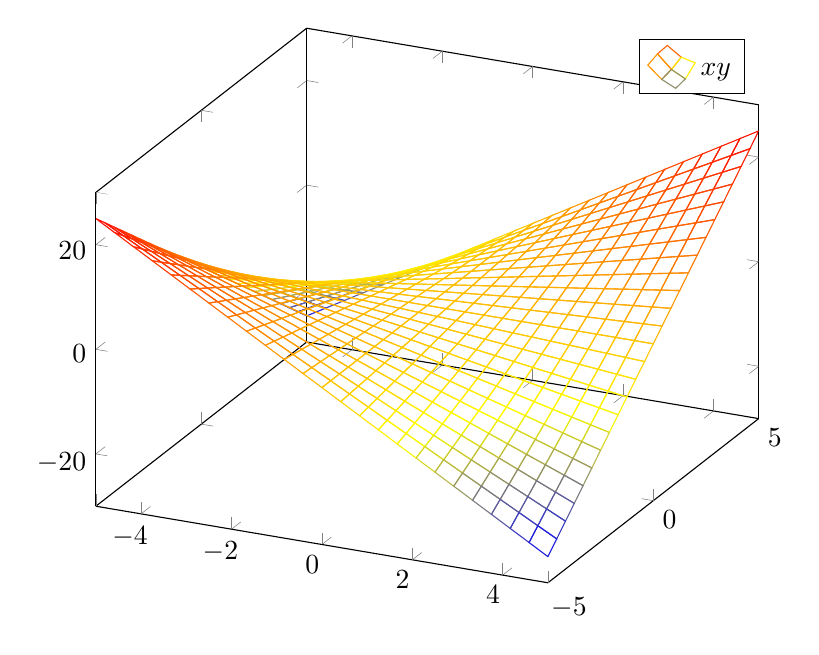
\begin{tikzpicture}
		\begin{axis}
			\addplot3[
			domain=-5:5,
			mesh
			]
			{x*y};
		\addlegendentry{\(xy\)}
		\end{axis}
	\end{tikzpicture}
\end{figure}


\begin{figure}[H]
	\centering
	% interesting graphs
	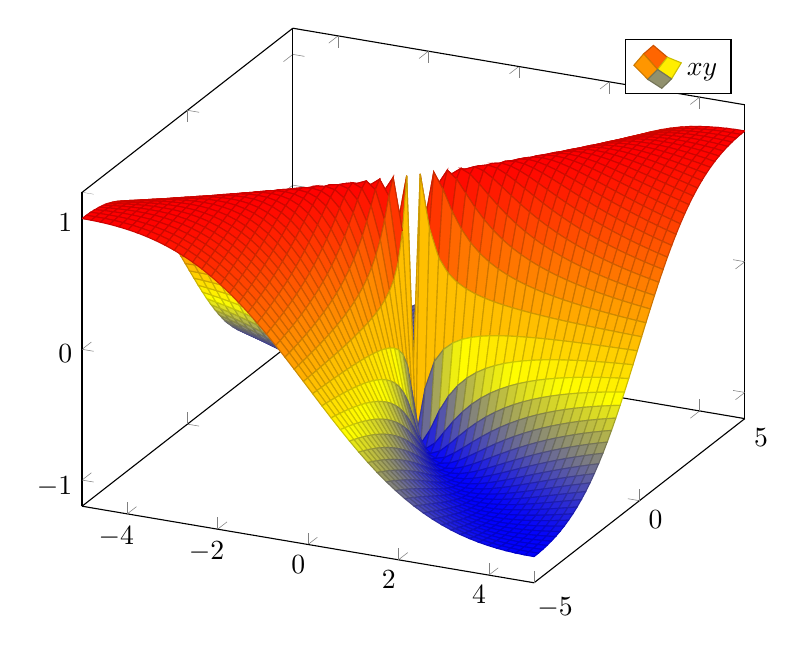
\begin{tikzpicture}
		\begin{axis}
			\addplot3[
			domain=-5:5,
			samples=50,
			surf
			]
			{2*x*y / (x*x + y*y)};
			\addlegendentry{\(xy\)}
		\end{axis}
	\end{tikzpicture}
\end{figure}

\subsection{Prerequisite Limits}
The sum of inequalities (absolutes). For $\epsilon > 0$, if
\[
	|x - x_0| < \epsilon \land |y - y_0| < \epsilon
\]
then
\[
	|x+y - (x_0+y_0)| = |x-x_0 + y-y_0| \leq |x-x_0| + |y-y_0| < 2 \epsilon
\]

The product of inequalities (absolutes). If
\[
	|x - x_0| < \frac{\epsilon}{2(|y_0| + 1)} \land |y-y_0| < \frac{\epsilon}{2(|x_0| + 1)} \land |x-x_0| < 1
\]
then
\[
	|xy - x_0y_0| < \epsilon
\]
\begin{proof}
	Consider
	\begin{align*}
		|xy - x_0 y_0| &\leq |xy - x y_0| + |x y_0 - x_0 y_0|\\
		&= |x(y-y_0)| + |y_0 (x-x_0)|\\
		&\leq |x| |y-y_0| + |y_0| |x-x_0|\\
		&< |x| \frac{\epsilon}{2(|x_0| + 1)} + |y_0| \frac{\epsilon}{2|y_0| + 1}\\
		&= \frac{\epsilon}{2} \left( \frac{|x|}{|x_0| + 1} + \frac{|y_0|}{|y_0|+1} \right)
	\end{align*}

	It is then simple to see that
	\[
		\frac{|y_0|}{|y_0| + 1} < 1
	\]
	and if $|x-x_0| < 1$,
	\[
		|x| - |x_0| \leq |x - x_0| \leq 1 \implies \frac{|x|}{|x_0| + 1} < 1
	\]

	So
	\[
		|xy-x_0y_0| < \frac{\epsilon}{2} \left( \frac{|x|}{|x_0| + 1} + \frac{|y_0|}{|y_0|+1} \right) < \frac{\epsilon}{2} 2 = \epsilon
	\]
\end{proof}


The quotients of inequalities (absolutes). If $y_0 \neq 0$ and
\[
	|y - y_0| < \min (\frac{|y_0|}{2}, \epsilon \frac{|y_0|^2}{2})
\]

then $y \neq 0$ and
\[
	\left|\frac{1}{y} - \frac{1}{y_0} \right| < \epsilon
\]
\begin{proof}
	Consider
	\begin{align*}
		\left| \frac{1}{y} - \frac{1}{y_0} \right| &= \left| \frac{y_0 - y}{y y_0} \right|\\
		&= \frac{|y-y_0|}{|y y_0|}\\
		&= \frac{|y - y_0|}{|y| |y_0|}\\
		&< \frac{\epsilon |y_0|^2}{2|y| |y_0|}\\
		&= \frac{\epsilon |y_0|} {2|y|}
	\end{align*}

	Notice that because
	\[
		|y-y_0| < \frac{|y_0|}{2}
	\]
	then
	\begin{align*}
		|y_0| - |y| &\leq |y_0 - y| = |y-y_0| < \frac{|y_0|}{2}\\
		\frac{|y_0|}{2} &< |y|\\
		\frac{|y_0|}{2|y|} &< 1
	\end{align*}
	therefore
	\[
		\left| \frac{1}{y} - \frac{1}{y_0} \right| < \frac{\epsilon |y_0|} {2|y|} < \epsilon
	\]
\end{proof}



\newpage
\section{Limits}

\begin{defn}{Definition of Limits}{}
	For the function $f(x)$ to have a limit $f(a)$ at point $a$ of value $f(a)$. We must have the following.

	Let $\epsilon > 0$, for any arbitrary epsilon. The function has a limit at $a$ if and only if no matter what $\epsilon$ is, there exists a $\delta > 0$ such that $\forall x, |x-a| < \delta$, that
	\[
		|f(x) - f(a)| < \epsilon
	\]
	then we can state that
	\[
		\lim_{x \to a} f(x) = f(a)
	\]
\end{defn}

The function's limit at a point is unique. (ie, if the function has two limits $a$ and $b$ at a point, then $a=b$)

We can limit both delta and epsilon to smaller values (or a smaller range). If delta is a smaller range, it automatically works even if epsilon is large, as we can still use the smaller delta range. If epsilon is a smaller range, then even if epsilon is greater, the delta used for the lowerbound of epsilon still works.

\begin{theorems}{The limit laws}{}
	Suppose that
	\[
		\lim_{x\to a} f(x) = l, \lim_{x\to a} g(x) = m
	\]
	then
	\[
		\lim_{x\to a} (f+g)(x) = l + m
	\]
	and
	\[
		\lim_{x \to a} (fg)(x) = lm
	\]
	and
	\[
		\lim_{x\to a} \frac{f}{g}(x) = \frac{l}{m}, m \neq 0
	\]
\end{theorems}
\begin{proof}
	The proof for the first (addition) and third (division) are very similar to the proof for the second, hence will not be shown.

	To prove the second, where
	\[
		\lim_{x \to a} f(x) = l, \lim_{x \to a} g(x) = m
	\]

	To show that $\lim_{x \to a} f(x)g(x) = lm$, select any $\epsilon > 0$.

	Let $\epsilon_1 = \min(1, \frac{\epsilon}{2(|m|+1)})$, and $\epsilon_2 = \frac{\epsilon}{2(|l|+1)}$. Consider the epsilon delta proof of the limit using $\epsilon_1$ and $\epsilon_2$.

	Suppose $\delta_1$ is the corresponding delta for $f(x)$, and $\delta_2$ is the corresponding delta for $g(x)$, then for
	\[
		|x - a| < \delta
	\]
	where $\delta = \min(\delta_1, \delta_2)$, so $\delta \leq \delta_1 \land \delta \leq \delta_2$, and
	\begin{align*}
		|f(x)-l| &< \epsilon_1\\
		|g(x)-m| &< \epsilon_2\\
	\end{align*}
	hence by the exercise (additional proof) this implies that
	\[
		|fg - lm| < \epsilon
	\]

	Thus the proof using the delta $\delta$ for the given epsilon $\epsilon$, near the point $a$.
\end{proof}

\begin{defn}{Lack of a limit}{}
	A function $f(x)$ does not have a limit $f(a)$ at $a$ if and only if:

	There exists an $\epsilon > 0$, such that for all $\delta > 0$, there exists a point $x$ where $|x - a| < \delta$, and
	\[
		|f(x) - f(a)| > \epsilon
	\]
\end{defn}

\subsection{Examples}
The limit
\[
	\lim_{x \to 0} \sin \left(\frac{1}{x}\right)
\]
does not exist.

\subsection{Limit Identities}
\begin{iden}{Limit operations}{}
    We have that
    \[
    \lim_{x \to a} f(x) = \lim_{h \to 0} f(a+h)
    \]

	The limit
	\[
		\lim_{x \to a} f(x) = l
	\]
	is valid if and only if
	\[
		\lim_{x \to a} f(x)-l = 0
	\]

	The expression
	\[
		\lim_{x \to 0} f(x) = \lim_{x \to a} f(x-a)
	\]
	always holds.

	For if $|h(x)| \leq M$ for $M \geq 0$, and
	\[
		\lim_{x\to a} f(x) = 0
	\]
	then
	\[
		\lim_{x \to a} f(x)g(x) = 0
	\]
\end{iden}

Define the lower and upper limit as
\begin{defn}{One-sided limits}{}
	The limit of a function $f$ at $a$ as approached from the right is
	\[
		\lim_{x \to a^+} f(a) = l
	\]
	if and only if
	\[
		\forall \epsilon > 0, \exists \delta > 0, \forall x, 0 < x - a < \delta \implies |f(x) - l| < \epsilon
	\]

	Similarly, the below limit replaces $0 < x - a < \delta$ with
	\[
		\forall x, -\delta < x - a < 0
	\]

	They are intuitively the two signs of the full limit. Moreover, the full limit implies the existences of the two signed limits, and vice versa, with the signed limited being equal implying the existence of the full limit.
\end{defn}

\begin{defn}{Codomain infinity limits}{}
	We define the limit of infinity
	\[
		\lim_{x \to a} f(x) = \infty
	\]
	by
	\[
		\forall N, \exists \delta > 0, \forall x, 0 < |x-a| < \delta \implies f(x) > N
	\]

	That is, for any large number $N$, there exists an interval around $a$ of size $2\delta$ where its image all land above the line $N$.
\end{defn}


\begin{defn}{Domain infinity limits}{}
	A function $f$ has a limit $l$ as $x$ approaches infinity when
	\[
	\forall \epsilon > 0, \exists N \in \mathbb{N}, \forall x > N, |f(x) - l| < \epsilon
	\]
	then we can say
	\[
	\lim_{x \to \infty} f(x) = l
	\]
\end{defn}

\begin{defn}{Infinity infinity limit}{}
	A function is said to
	\[
		\lim_{x \to \infty} f(x) = \infty
	\]
	if for any $N$, there exists some number $M$ such that $\forall x > M$, $f(x) > N$.

	We can also impose the restriction that $N > 0$ and $M > 0$.

	This statement also applies for $-\infty$ and the combination of the two.
\end{defn}


\begin{iden}{Infinity limits substitutions}{}
	For any function $f$, the following two limits, if exists, are equal
	\[
	\lim_{x \to 0^+} f(1/x) = \lim_{x \to \infty} f(x)
	\]

	Intuitively, this states that the limit of $f(1/0)$ from the right is equivalent to the limit $f(\infty)$ towards $\infty$.
\end{iden}

\newpage
\section{Continuity}
\begin{defn}{Continuity}{}
	A function $f$ is continuous at $x=a$ if and only if the following limit exists and
	\[
		\lim_{x \to a} f(x) = f(a)
	\]

	Note that $f(a)$ must exist/defined as well. We can use a function extension to make it continuous.
\end{defn}

Continuity simply refers to the idea that the function has a well-defined limit at a point.
The class of polynomials is continuous at every point. The class of rational functions is also continuous at every point of its domain.

\begin{theorems}{Continuity laws}{}
	If $f$ and $g$ are functions that are continuous at $x=a$, then by the limit laws:
	\[
		f+g, fg, \frac{f}{g} \land g(a) \neq 0
	\]
	are all continuous at $x=a$.
\end{theorems}


\begin{theorems}{Continuity Function Composition}{}
	If $g$ is continuous at $x=a$, and $f$ is continuous at $x=g(a)$, then
	\[
		\lim_{x \to a} f(g(x)) = f(g(a))
	\]
	is also continuous at $x = a$, given that the function composition is possible.
\end{theorems}

\begin{proof}
	This is a proof for the function composition continuity. Suppose that $g$ is continuous at $a$ and the function $f$ is continuous. To show that the limit
	\[
		\lim_{x \to a} f(g(x))
	\]
	both exists and is continuous, consider any $\epsilon > 0$.

	Because $f$ is continuous at $g(a)=y$, then $\lim_{x\to y} f(x) = f(y)$, and for the epsilon $\epsilon$, there exists a $\delta_1$ such that
	\[
		\forall x, 0 < |x - y| < \delta_1, |f(x) - f(y)| < \epsilon
	\]

	Now because $g$ is continuous around $a$ (with $g(a)$), then for any $\epsilon_1 = \delta_1$, there exists $\delta > 0$ such that
	\[
		\forall x, 0 < |x - a| < \delta, |g(x) - g(a)| < \epsilon_1 = \delta_1
	\]

	Notice that this implies
	\[
		\forall x, 0 < |x - a| < \delta, |g(x) - y| < \delta_1, |f(g(x)) - f(y)| < \epsilon, |f(g(x)) - f(g(a))| < \epsilon
	\]
	hence the limit exists at $x=a$ with $f(g(a))$. This is also the condition for continuity.
\end{proof}

A function $f$ is continuous on an interval $(a, b)$ iff $\forall x \in (a,b)$, $f$ is continuous at $x$.

A function is continuous for the real numbers if it is continuous on the interval $(-\infty, \infty)$.


\begin{theorems}{Positive/negative intervals}{}
	If a function $f$ is continuous at $a$, and $f(a) > 0$. There exists some interval where for all $x$ in that interval, $f(x) > 0$.

	And for the negatives, if $f(a) < 0$, then there exists some interval where for all $x$ within, $f(x) < 0$.
\end{theorems}
\begin{proof}
	This is trivial. The hint is to use the $\delta$ in the formal limit proof as the interval and set $\epsilon = f(a) > 0$.
\end{proof}

\subsection{Continuity Theorems}
The graph of a continuous function that starts below the axis line and ends above it must cross the axis at some point. More formally, this is
\begin{theorems}{Axis crossing}{}
	If $f$ is a continuous function across the interval $(c, d)$, with
	\[
		c < a < b < d
	\]
	and
	\[
		f(a) < 0 < f(b)
	\]
	then there exists some $x \in (a,b)$ such that $f(x) = 0$
\end{theorems}
Notice that $f(x)$ must be continuous across the entire interval. Otherwise, say $f = \frac{1}{x}$, then this theorem does not hold.

To generalize this, notice both that $y = 0$ is not special, and we could also have $f(b) > 0 > f(a)$. Moreover
\begin{theorems}{Intermediate value theorem}{}
	If a continuous function $f$ on an interval ($a$ and $b$) takes on two values ($c$ and $d$), then throughout the interval $[a, b]$, it must take on all values from $[c, d]$.
\end{theorems}
\begin{proof}
	The proof of this theorem requires some property of the real numbers, property that we will not describe.
\end{proof}

The intermediate value theorem is defined only for the real numbers, for it immediately guarantees the existence of square roots (a property that the rational numbers do not have)
\begin{corollary}
	Every positive real number has a real number square root
\end{corollary}
\begin{proof}
	Consider the function $f(x) = x^2$. Suppose for $a > 0$, let the interval be $[0, \max(1, a)]$.

	Notice that $f(0) = 0 < a < f(\max(1, a))$, therefore by the intermediate value theorem ($f$ is continuous), there exists a value $x \in [0, \max(1, a)]$ such that $f(x) = x^2 = a$. Hence $x$ is the real square root of $a$.
\end{proof}

\subsection{Continuity Laws}
\begin{defn}{Continuity on a closed interval}{}
	We say that a function $f$ is continuous on a closed interval $[a, b]$ when it is continuous on $(a, b)$ and
	\[
		\lim_{x \to a^+} f(x) = f(a) \land \lim_{x \to b^-} f(x) = f(b)
	\]
\end{defn}



The theorem for where there exists an interval around the continuous point where the function values have the same sign applies to left/right continuities as well, albeit at around the signed point.

\begin{theorems}{Continuous extension}{}
	If $f$ is continuous on the interval $[a, b]$, then there exists an extension $g(x)$, namely
	\[
		g(x)= \begin{cases}
			f(x) & x \in [a,b]\\
			f(a) & x < a\\
			f(b) & x > b
		\end{cases}
	\]
	where $g(x)$ is continuous for all reals.

	This is because the extension is continuous at the boundary $x=a$ and $x=b$ as well, for those points have one part limit from the interval, and the other part limit from the constant extension.

	This does not work for open intervals $(a, b)$.
\end{theorems}

\subsection{Additional Continuity Theorems}

Followup from the IVT.
\begin{theorems}{Bounded value theorem}{}
	For a function $f$ that is continuous from $[a, b]$, the function will be bounded between this domain by:
	\[
		\exists N, \forall x \in [a,b], f(x) \leq N
	\]

	This tells us there is both an upper and lower bound to the function (maximum and minimum) in the continuous domain.

	Moreover, a stronger theorem (the extreme value theorem) suggests that the maximum and minimum bounds are values of the function:
	\[
		\exists y_1, y_2 \in [a,b], \forall x \in [a,b], f(y_1) \leq f(x) \leq f(y_2)
	\]
\end{theorems}
\begin{proof}
	No proof lets go.
\end{proof}

Here are some polynomial theorems.

\begin{lemmas}{Polynomial dominant}{}
	For $p_n(x)$,
	\[
	\lim_{x \to \infty} p_n(x) = \infty
	\]
\end{lemmas}
\begin{proof}

	Let
	\begin{align*}
		p_n(x) &= x^n + a_{n-1} x^{n-1} + \dots + a_0\\
		&= x^n \left( 1 + \frac{a_{n-1}}{x^1} + \dots  + \frac{a_0}{x^n} \right)
	\end{align*}

	Consider the bound of the rhs fractions, if we let $x > M = \max(1, 2n|a_{n-1}|, \dots, 2n|a_0|)$,
	\begin{align*}
		\left| \frac{a_{n-1}}{x^1} + \dots  + \frac{a_0}{x^n} \right| &\leq \frac{|a_{n-1}|}{|x|} + \dots + \frac{|a_0|}{|x^n|}\\
		&< \frac{1}{M} (|a_{n-1}| + \dots + |a_0|)\\
		&= \frac{1}{2nM} (2n|a_{n-1}| + \dots + 2n|a_0|)\\
		& \leq \frac{1}{2nM} (nM)\\
		&= \frac{1}{2}
	\end{align*}

	Hence because
	\begin{align*}
		\frac{a_{n-1}}{x^1} + \dots  + \frac{a_0}{x^n} &> -\frac{1}{2}\\
		p_n(x) =  x^n \left( 1 + \frac{a_{n-1}}{x^1} + \dots  + \frac{a_0}{x^n} \right) &> x^n (1 - \frac{1}{2})\\
		&= \frac{1}{2} x^n
	\end{align*}
	So by also letting $x > 2N$, we have
	\[
	\frac{1}{2}x^n > \frac{1}{2} x > N
	\]

	Our $M$ for a given $N$ is therefore
	\[
	M = \max(2N, 1, 2n |a_{n-1}|, \dots, 2n |a_0|)
	\]
	So that $\forall x > M \implies p_n(x) > N$.

\end{proof}

\begin{theorems}{Odd polynomial roots}{}
	For an $n$th degree polynomial $p_n(x)$. If $n$ is odd, then there exists some $x$ such that
	\[
	p_n(x) = 0
	\]
	This is because $p_n(\infty) > 0$ and $p_n(-\infty) < 0$.
\end{theorems}
\begin{proof}
	It is easy to see that if
	\begin{align*}
		\lim_{x \to \infty} p(x) &= \infty\\
		\lim_{x \to -\infty} p(x) &= -\infty
	\end{align*}
	then by the intermediate value theorem, since $-\infty < 0 < \infty$, there exists $-\infty < x < \infty$ such that $p(x) = 0$.
\end{proof}

\begin{theorems}{Even polynomials}{}
	For an $n$th degree polynomial $p_n(x)$ for even $n$. There exists a number $m$ such that
	\[
	\forall x, p_n(x) = c \geq m
	\]
	has a solution, but not if $c < m$
\end{theorems}
\begin{proof}
	We will first show that the polynomial has a minimal, and let it be $m$.

	Consider the value $p_n(0)$, and since $p_(\pm \infty) = \infty$, there exists $b^-$ and $b^+$ such that
	\begin{align*}
		\forall x < b^- < 0&, p_n(x) > p_n(0)\\
		\forall x > b^+ > 0&, p_n(x) > p_n(0)
	\end{align*}

	Hence consider the interval $[b^-, b^+]$, by the extreme value theorem, there exists a minimal value $p_n(y)$ such that
	\[
		\forall x \in [b^-1, b^+], p_n(x) \geq p_n(y)
	\]
	namely, $p_n(0) \geq p_n(y)$. This also holds outside the interval, for all $x$ outside, $p_n(x) > p_n(0) \geq p_n(y)$. Hence let $m = p_n(y)$, denoting the global minimum of the polynomial.

	For all $c < m$, the function does not have a solution because its range is greater or equal to $m$, and thus there are no $x$ such that $p_n(x) < m$.

	For all $c \geq m$, because $p_n(\infty) = \infty$, there exists a $b > 0$ such that $\forall x > b, p_n(x) > c$. Therefore consider the interval $[y, b+1]$ with range $[m, p_n(b+1)]$. Because
	\[
		m \leq c < p_n(b+1)
	\]
	, by the IVT, there exists some value $y < x < b+1$ such that $p_n(x) = c$. If the interval is ordered in reverse, simply flip the intervals and this still holds. Hence there always exists some solution for $p_n(x) = c$.
	% Use the idea that p_n(x) goes to infinity to find a closed interval where everything outside is greater. Then use the extreme value theorem to find the min

	% Use the min to prove that no solution exists below min, and solutions must exist above min (using IVT)
\end{proof}

The proof of the IVT is complicated and will not be examined.








\newpage
\section{Multivariate Limits and Continuity}
We say a two dimensional function has a limit at some point if for any curve on the xy plane that passes through that point, their limits exist and are equal.

\begin{defn}{2D function limits}{}
    A function $f(x, y)$ has a limit $l$ at $(a, b)$ if for all $\epsilon > 0$,
    \[
        \exists \delta > 0, \forall (x,y), 0 < |(x,y)-(a,b)| < \delta \implies |f(x,y) - l| < \epsilon
    \]

    The intuition is that for any two planes above and below the limit, we can choose a disc of some radius around $(a, b)$ such that the image of the disk is within the two planes.

    Alternatively, we can merely find a square around $(a,b)$, in that
    \[
        \forall x, 0 < \max(|x - a|, |y - b|) < \delta
    \]
    where the image is contained within the plane.

    Then we can state that
    \[
        \lim_{(x,y) \to (a, b)} f(x,y) = l
    \]
\end{defn}

Often, the value that a function approaches at a point depends on the direction at which it is approached (straight line, parabola). Therefore we must use the direction independent limit definitions.

\subsection{Examples}
The function
\[
    g(x, y) = \frac{x^2 y}{x^4 + y^2}
\]
does not have a limit at $(0, 0)$. This is because
\[
    \forall x, g(x, cx^2) = \frac{c}{1+c^2}
\]
which can be positive, negative, or zero depending on the $c$ chosen. The formal proof utilize this by selecting a pair $(x, cx^2)$ within the $\delta$ disk with an appropriate $c$. If the limit were to be positive, selecting $c$ to be negative will yield an output that is also negative --- setting $\epsilon = l$ will show that the limit does not work. Similarly for a negative limit. If the limit is zero, let $\epsilon = 0.1$, and let $c = \frac{1}{2}$ to which the function output would be $0.4 > \epsilon$.

\subsection{Continuity Theorems}

\begin{defn}{2D continuity}{}
    A function $f(x,y)$ is said to be continuous at $(a, b)$ when
    \[
        \lim_{(x,y) \to (a, b)} f(x, y) = f(a,b)
    \]

    This implies that the limit of the function at $(a,b)$ is equal to the value of the function at $(a, b)$.
\end{defn}

The continuity laws essentially translate line-by-line from the single variable case:
\begin{theorems}{2D continuity laws}{}
    For the continuous functions $f$ and $g$. Their sum and product are continuous. Their quotient $\frac{f}{g}$ is also continuous on the domain where $g(x,y)$ is not zero.
\end{theorems}




\begin{defn}{Separately Continuous}{}
    A function $f(x, y)$ is separately continuous when both $\forall b, f(x, b)$ and $\forall x, f(a, y)$ are continuous functions of $x$ or $y$.

    This means that the function $f$ is continuous across any slices parallel to the axis.

    A separately continuous function need not to be continuous in the 2D plane. But any continuous two functions are separately continuous
\end{defn}

\begin{defn}{Generalized limits}{}
    A function $f \colon \mathbb{R}^n \to \mathbb{R}$ has a limit $l$ at $\vec{a}$ when
    \[
        \forall \epsilon > 0, \exists \delta > 0, \forall \vec{x}, 0 \leq |\vec{x} - \vec{a}| < \delta \implies |f(\vec{x}) - l| < \epsilon
    \]
\end{defn}

% write the proof that g(f(x, y)) is continuous if f and g are too
Elementary functions are continuous.

\begin{theorems}{2D continuity composition}{}
    Let $f \colon A \to \mathbb{R}^2$ and $g \colon B \to \mathbb{R}$. If both $f$ and $g$ are continuous on their domain, and if $f(A) \subset B$, then
    \[
        h = g \circ f
    \]
    is continuous on the domain $A$.
\end{theorems}

\paragraph{Example} For example
\[
    f(x, y) = x - y = g(x, h(-1, y))
\]
where $g(a, b) = a + b$ and $h(a, b) = ab$. Because both $g$ and $h$ are continuous, the composition is also continuous.




\newpage
\section{Differentiation}
\begin{defn}{Differentiation}{}
    A function $f$ is differentiable at $x=a$ when the limit
    \[
        \lim_{h \to 0} \frac{f(a+h) - f(a)}{h}
    \]
    exists.

    If the limit exists, denote this limit by $f'(a)$.
\end{defn}


\begin{theorems}{Continuity Relation}{}
    If a function $f$ is differentiable at a point $x=a$, then the function is continuous at $f(a)$.
\end{theorems}


If a function is differentiable throughout its domain, the say this function is differentiable.

\begin{theorems}{Sum, Product of derivatives}{}

    Suppose that $f$ and $g$ are differentiable at $x=a$, then
    \begin{align*}
        (f+g)'(a) &= f'(a) + g'(a)\\
        (fg)'(a) &= f'(a) g(a) + f(a) g'(a)
    \end{align*}
\end{theorems}
\begin{proof}
    These proofs are very simple.
\end{proof}

\subsection{Linear Approximation}

A linear approximation $l(x)$ to a function near $x=a$ is
\[
    l(x) = f(a) + f'(a) (x-a)
\]
And let the error $h(x)$ be
\[
    h(x) = f(x) - l(x)
\]

We note that the linear error function $h$ approaches zero faster than the distance, namely
\[
    \lim_{x\to a} \frac{h(x)}{x-a} = 0
\]
when $f(x)$ is differentiable at $x=a$.

This implies the statement that
\[
    \lim_{x \to a} h(x) = 0
\]
This can be used to prove that $f$ is continuous at $x=a$ if it is differentiable at that point.

\begin{lemmas}{}{}
    If for some point $a$,
    \[
        f(x) = f(a) + m (x-a) + h(x)
    \]
    and
    \[
        \lim_{x\to a} \frac{h(x)}{x-a} = 0
    \]

    Then $f$ is differentiable at $x=a$ and $f'(a) = m$. And vice versa (if $f$ is differentiable, the above two expressions are defined).
\end{lemmas}
\begin{proof}
    Consider
    \begin{align*}
        \lim_{x \to a} \frac{f(x) - f(a)}{x-a} &= \lim \frac{f(a) + m(x-a) + h(x) - f(a)}{x-a}\\
        &= \lim m + \frac{h(x)}{x-a}\\
        &= m = f'(a)
    \end{align*}
\end{proof}

To show that the function is not differentiable at a point $x=a$, it suffices to show that the differential quotient limit does not exist.

\subsection{Multivariate differentiation}

\begin{defn}{Higher Order derivatives}{}
    Define the $k$th derivative to be
    \[
        f^{(k+1)} = (f^{(k)})'
    \]
\end{defn}

We can use the first derivative to prove that the second derivative exists/not exists.

To generalize differentiation for multivariate functions, a function is differentiable with derivative Jacobian $J_f$ at $X = A$ when
\[
    f(X) = f(A) + J_f (X-A) + E(X)
\]
and
\[
    \lim_{X \to A} \frac{E(X)}{|X-A|} = 0
\]

When $X$ are 2D vectors, $J_f$ is the gradient row vector pointing to the direction of steepest ascent.

Vice versa if we could find such a linear approximation and suitable $E(X)$ error function, the jacobian will be the matrix $J_f$.

\begin{defn}{Partial derivatives}{}
    The partial derivative of $f(X)$ against $X_i$ is
    \[
         \partial_{X^i} f = \frac{\partial f}{\partial X^i} (A) = \lim_{h \to 0} \frac{f(A + h X^i) - f(A)}{h}
    \]

    The partial derivative exists when the limit exists.
\end{defn}

\begin{theorems}{}{}
    If the function $f(X)$ is differentiable at $X=A$, then
    \[
        \partial_{X^j} f = \frac{\partial f}{\partial X^j} = {J_f}^i {}_{j}
    \]
    ie, the column $j$ of the Jacobian $J_f$.

    The intuition is to set all but one axis to be constant at the limit, and apply the linear approximation definition to find the partial derivative limit.

    Conversely, if any partial derivative does not exist, the function must not be differentiable at that point.
\end{theorems}

When the multivariate function is scalar valued, the Jacobian is also called the gradient row vector:
\[
    J_f = \nabla f(A)
\]


\begin{theorems}{Partial Derivatives}{}
    For a function $f(X)$. If all of its partial derivatives as a multivariate function exists everywhere and is continuous at $A$, then the function $f$ is differentiable at $A$.
\end{theorems}

\begin{defn}{Directional Derivatives}{}
    Define the directional derivative of a differentiable vector-valued function $f(X)$ along the unit direction $v$
    \[
        \nabla_v f(X) = \partial_{v} f(X) = v \cdot \nabla f(X) = \lim_{t \to 0} \frac{f(X+t v) - f(X)}{t}
    \]

    To prove this relation, simply substitute in the limit the linear approximation along the direction $f(X + t v)$.
\end{defn}

Notice that
\[
    |\partial_v f(X)| = |\nabla f(X) \cdot v| \leq |\nabla f(X)|
\]
The directional derivative is maximized when $v = |\partial f(X)|$. This shows that the gradient is the steepest line of ascent.

\begin{defn}{Chain Rule}{}
    For a function $f(X)$ differentiable at $g(t)$, for a differentiable $g(x)$ at $x=t$, then the function $f(g(x))$ is differentiable at $x=t$ with
    \[
        \left. \frac{d}{dx} f(g(x)) \right\rvert_{x = t}  = \nabla f(g(t)) \cdot g'(t)
    \]

    We denote the vector valued function $g(x)$ as a parameterized curve.

    The directional derivative is a special case where $g(x) = a + v x$, for the directional unit vector $v$, where $g'(x) = v$.
\end{defn}
\begin{proof}
    Consider the linear approximation of $f(g)$ at $x+t$. Because both $f$ and $g$ are differentiable,
    \[
        f(g(x + t)) = f(g(x+t) - g(x) + g(x)) = f(g(x)) + \nabla f(g(x)) \cdot h + E_1(h)
    \]
    where $h = g(x+t) - g(x)$, and $\lim_{h \to 0} \frac{E_1(h)}{|h|} = 0$.

    Notice that because $g$ is differentiable
    \begin{align*}
        h &= g(x + t) - g(x)\\
        &= g'(x) t + E_2(t)
    \end{align*}

    Then
    \[
        f(g(x+t)) = f(g(x)) + \nabla f(g(x)) \cdot g'(x) t + \nabla f(g(x)) \cdot E_2(t) + E_1(h)
    \]
    with the last two terms approaching zero faster than linear. Hence, the derivative is
    \[
        \frac{d}{dx} f(g(x)) = \nabla f(g(x)) \cdot g'(x)
    \]

\end{proof}

The chain rule is a special case of the definition of the general full derivative $\frac{d}{dx}$ on multivariate functions.


\subsection{Differentiation identities}
Here are some useful gradient rules, assuming that $x = \vec{x}$
\begin{itemize}
    \item $\nabla (|x|) = \frac{x}{ |x| }$
    \item $\nabla (a \cdot x) = a$
    \item If $f$ and $g$ are both differentiable (have gradients) at $A$,
    \begin{align*}
        \nabla (f+g) (A) &= \nabla f(A)  + \nabla g(A)\\
        \nabla (fg)(A) &= f(A) \nabla g(A) + g(A) \nabla f(A)
    \end{align*}
    and both $f+g$ and $fg$ are differentiable at $A$.
\end{itemize}

\begin{theorems}{Chain rule linear approximation extras}{}
    To show that
    \[
        \lim_{t \to 0} \frac{E_1(h)}{t} = 0
    \]
    with
    \begin{align*}
        \lim_{h \to 0} \frac{E_1(h)}{h} &= 0\\
        h &= g(x+t) - g(x)
    \end{align*}

    Consider
    \begin{align*}
        \lim_{t \to 0} \frac{E_1(h)}{t} &= \lim_{t \to 0} \frac{E_1(h)}{h} \frac{h}{t}\\
        &=  g'(t) \lim_{t \to 0} \frac{E_1(h)}{h}\\
        &= g'(t) \left[ \lim_{h \to (\lim_{t \to 0} h)} \frac{E_1(h)}{h} \right]\\
        &= g'(t) \left[ \lim_{h \to 0} \frac{E_1(h)}{h} \right]\\
        &= 0
    \end{align*}
\end{theorems}

To show that a function is not differentiable at a point, we can prove by contradiction in deriving an explicit formula for the directional derivative (using limits), then using the identity
\[
    \nabla_u f = \nabla f \cdot u
\]
to show that the two methods of directional derivatives does not equal.

\newpage
\section{Differentiation Theorems}

\begin{theorems}{Mean value theorem}{}
    For a continuous function on $[a, b]$, where $f$ is differentiable on $(a,b)$. Then there exists a point $y$, where $f'(y)$ is the slope of the line between the endpoints:
    \[
        \exists y \in (a,b), f'(y) = \frac{f(b)-f(a)}{b-a}
    \]
\end{theorems}
\begin{proof}
    The equation for the line between the endpoints is
    \[
        l(x) = f(a) + \frac{f(b)-f(a)}{b-a} (x-a)
    \]

    Define the error between the line and function to be
    \[
        h(x) = f(x) - l(x)
    \]
    we now only need to show that at some point $y \in (a,b)$, $h'(y)=0$.

    Notice that
    \[
        h(a) = 0, \quad h(b) = 0
    \]
    with $h(x)$ being continuous on the closed interval $[a, b]$. Therefore by the EVT, $h(x)$ has a local extrema at some point $y\in(a,b)$.

    If the both the extremas are at the endpoints, then the error function is simply $h(x) = 0$, so the original function $f(x) = l(x)$, and itself is also a straight line.

    Otherwise, at the extrema, $h'(y) = 0$.
\end{proof}

\begin{theorems}{Cauchy mean value theorem}{}
    Suppose $f$ and $g$ are continous on $[a,b]$, and are differentiable on $(a,b)$, then there exists a point $y \in (a,b)$ such that
    \[
        (f(b)-f(a)) g'(y) = (g(b)-g(a)) f'(y)
    \]

    Or when $g'(y) \neq 0$ and $g(b) - g(a) \neq 0$,
    \[
        \frac{f(b) - f(a)}{g(b) - g(a)} = \frac{f'(y)}{g'(y)}
    \]

    This implies that for the parametric curve defined by $(f(t), g(t))$, there exists a tangent curve with the same slope as the secant from the curve's endpoints. This geometrical intuition will only hold when both $f'(y) \neq 0$ and $g'(y) \neq 0$, however.
\end{theorems}
\begin{proof}
    Define
    \[
        h(x) = (f(b)-f(a))g(x) - f(x)(g(b)-g(a))
    \]
    with
    \[
        h(a) = f(b)g(a)-f(a)g(b), \quad h(b) = f(b)g(a)-f(a)g(b)
    \]

    Hence there exists a point $y \in (a,b)$, where $h'(y) = 0$, for the endpoints are the same. And at such point, Cauchy's mean value theorem holds.

    If both the extremas are at the endpoints, then forall $x$, $h(x) = 0$. Hence $\forall y \in (a,b), h'(y) = 0$, and the proof follows.

\end{proof}



Here is a helper theorem to better understand the above theorems.
\begin{theorems}{Rolle's Theorem}{}
    For a function $f$ that is continuous on $[a,b]$, and differentiable on $(a,b)$, then
    \[
        \exists y \in (a,b), f'(y) = 0
    \]
    when $f(a) = f(b)$.
\end{theorems}
\begin{proof}
    By the extreme value theorem, $f$ has a local maximum at $y$, where
    \[
        \forall x, f(y) \geq f(x)
    \]

    Assume that $y$ or at least one extrema is not at $a$ or $b$. Then
    \[
        \frac{f(y+h) - f(y)}{h} = \begin{cases}
            \leq 0 & h > 0\\
            \geq 0 & h < 0
        \end{cases}
    \]
    and because $f$ is differentiable at $y$, the left and right limit must agree, and thus $f'(y) = 0$.

    If both extremas are at $a$ and $b$, then $f(x) = 0$, and it is obviously that for all $x \in (a,b)$, $f'(x) = 0$.
\end{proof}


\begin{theorems}{L'Hopital's rule}{}
    Suppose $f(x)$ and $g(x)$ are differentiable functions at zero and
    \[
        \lim_{x \to 0} f(x) = 0, \quad \lim_{x\to 0} g(x) = 0
    \]

    Moreover, if
    \[
        \lim_{x \to 0} \frac{f'(x)}{g'(x)} = l
    \]

    Then
    \[
        \lim_{x \to 0} \frac{f(x)}{g(x)} = l
    \]

    This implies that the limit of the quotient between the derivatives equals the quotient itself.
\end{theorems}
\begin{proof}
    Extend $f(0) = 0$ and $g(0) = 0$. The simple proof (assuming that $f'(x)$ is continous at $x=0$) is
    \begin{align*}
        \frac{f(x)}{g(x)} &= \frac{f(x) - f(0)}{g(x) - g(0)}\\
                          &= \frac{f'(0)}{g'(0)}
    \end{align*}
    and applying the various limits.

    More generally, using the cauchy mean value theorem
    \begin{align*}
        \frac{f(x)}{g(x)} &= \frac{f(x) - f(0)}{g(x) - g(0)}\\
                          &= \exists \alpha \in (0, x), \frac{f'(\alpha)}{g'(\alpha)}\\
    \end{align*}
    assuming that $g(x) - g(0) \neq 0$ and $g'(\alpha) \neq 0$.


    But $\alpha \to 0$ when $x \to 0$, hence at the limit $x \to 0$
    \[
        \lim_{x\to 0} \frac{f(x)}{g(x)} = \lim_{x\to 0}\frac{f'(x)}{g'(x)}
    \]

    Precisely, forall $\epsilon > 0$, there exists a $\delta > 0$, such that
    \[
        \forall x, 0 < |x| < \delta \implies \left|\frac{f'(x)}{g'(x)} - l\right| < \epsilon
    \]

    Consider, $\forall x, 0 < |x| < \delta$, there exists a $0 < \alpha < |x|$ where
    \[
        \frac{f'(\alpha)}{g'(\alpha)} = \frac{f(x)}{g(x)}
    \]

    but $0 < |\alpha| < |x| < \delta$, so
    \[
        \left|\frac{f(x)}{g(x)} - l \right| = \left|\frac{f'(\alpha)}{g'(\alpha)} - l \right| < \epsilon
    \]

    This shows that
    \[
        \lim_{x \to 0} \frac{f(x)}{g(x)} = l
    \]
\end{proof}

\begin{theorems}{Generalized L'Hopital's Rule}{}
    For continuous functions $f(x)$, $g(x)$, which are also differentiable.

    \paragraph{(1)} If
    \begin{align*}
        \lim_{x \to a} f(x) &= \lim_{x \to a} g(x) = 0
    \end{align*}
    and
    \[
        \lim_{x \to a} \frac{f'(x)}{g'(x)} = \infty
    \]

    Then
    \[
        \lim_{x \to a} \frac{f(x)}{g(x)} = \infty
    \]

    \paragraph{(2)} If
    \[
        \lim_{x \to \infty} f(x) = \lim_{x \to \infty} g(x) = 0
    \]
    and
    \[
        \lim_{x \to \infty} \frac{f'(x)}{g'(x)} = l
    \]

    Then
    \[
        \lim_{x \to \infty} \frac{f(x)}{g(x)} = l
    \]
\end{theorems}
\begin{proof}
    Similar to the specialized proof
\end{proof}

\newpage
\section{Multivariate properties}
\begin{defn}{Critical Points}{}
    For a multivariate scalar valued function $f$, a critical point $a$ is a point where
    \[
        \nabla f(a) = 0
    \]
    that is, the best linear approximation around a critical point is simply $l(x)=f(a)$.
\end{defn}

\begin{defn}{Local Extremas}{}
    A local minimum $a$ is a point where
    \[
        \exists \delta > 0, |x - a| < \delta \implies f(a) \leq f(x)
    \]
    Intuitively, this states that a within a small area around $a$, $f(a)$ is a minimum.

    Similarly is the definition for a local maximum.
\end{defn}

For a differentiable function, a local minimum or maximum must be a critical point (we can prove this by noticing that all directional derivatives are zero by Rolle's Theorem, hence the gradient is zero). The converse is \textbf{not} true.

To check for a local minimum/maximum via critical points, we conduct the seconderivative test using the Hessian matrix $H$. In 2D, the matrix is
\[
    H = \begin{bmatrix}
        \partial_x \partial_x f & \partial_x \partial_y f\\
        \partial_y \partial_x f & \partial_y \partial_y f
    \end{bmatrix}
\]
with the condition being that $\det H = 0$. NOT TESTED.

\subsection{Inverses}
A function is invertible if and only if it is a one to one mapping.
\begin{defn}{Bijection}{}
    A function is bijective when
    \[
        \forall x, y, f(x) = f(y) \implies x = y
    \]
    and that it is surjective.
\end{defn}

All increasing/decreasing functions are bijective and invertible. A function is increasing/decreasing within a interval will also be invertible.
\begin{defn}{Increasing function}{}
    An increasing function, monotonic function is one where
    \[
        \forall a, b, a < b \implies f(a) < f(b)
    \]
\end{defn}

Not all one-to-one functions are either increasing or decreasing. But all one-to-one functions which are continuous on an interval must be either increasing or decreasing.

\begin{theorems}{Properties of inverses}{}
    If $f$ is continuous and invertible (one-to-one) on an interval, then $f^{-1}$ will also be continuous on the domains defined.

    Similarly, $f^{-1}$ will be differentiable where
    \[
        \forall b, f'(f^{-1}(b)) \neq 0
    \]
\end{theorems}

\begin{theorems}{Derivative of inverses}{}
    For an invertible function $f$, where $g = f^{-1}$
    \[
        g'(y) = \frac{1}{f'(g(y))}
    \]
    This is intuitive for we can simply mirror the derivatives.

    This only holds when $f'(g(y)) \neq 0$.
\end{theorems}
\begin{proof}
    If both $f$ and $g$ are differentiable, simply apply the chain rule on
    \[
        \frac{d}{dy} f(g(y)) = \frac{d}{dy} y
    \]
    and rearrange.

\end{proof}
This shows that if $f(x)$ is a continuous invertible function in an interval $I$, and $\exists a$ where
\[
    f'(f^{-1}(a)) = 0
\]
then $f^{-1}$ must not be differentiable at $a$.

\subsection{Extras, Proofs}
To show that if $f(x,y)$ is continuous at $(a,b)$, and both partials are continuous in the 2D case around $(a,b)$, then the function is differentiable at the point.

Consider the error function
\[
    E(h, k) = f(a+h, b+k) - f(a,b) -h \partial_x f(a,b) - k \partial_y f(a,b)
\]
we are attempting to show that given the above conditions, then
\[
    \lim_{(h,k) \to (0,0)} \frac{E(h,k)}{|(h,k)|} = 0
\]
for then our partial creates a good enough linear approximation at $(a,b)$.

Then by the mean value theorem,
\begin{align*}
    \exists u_1 \in (a, a+h), &f(a+h, b+k) - f(a, b+k) = h f_x(u_1, b+k)\\
    \exists u_2 \in (b, b+k), &f(a, b+k) - f(a, b) = k f_y(a, u_2)
\end{align*}

Therefore, by substituting into the error function, we have
\begin{align*}
    E(h, k) &= h (f_x(u_1, b+k) - f_x(a,b)) + k(f_y(a, u_2) - f_y(a,b))
\end{align*}

Therefore
\begin{align*}
    \left| \frac{E(h,k)}{|(h,k)|} \right| &= \frac{|h| |f_x(u_1, b+k) - f_x(a,b)| + |k| |f_y(a, u_2) - f_y(a,b)|}{|(h,k)|}\\
    &\leq |f_x(u_1, b+k) - f_x(a,b)| + |f_y(a, u_2) - f_y(a,b)| < \epsilon \qquad \text{for } |h| \leq |(h,k)|
\end{align*}

Because $f_x(a,b)$ is continuous, for $\epsilon_1 = \frac{\epsilon}{2} > 0$, there exists $\delta_1 > 0$ such that
\[
    \forall |(h,k)| < \delta_1 \implies |f_x(a+h, b+k) - f_x(a,b)| < \epsilon_1
\]
(assuming that we use this delta bound) then because $a < u_1 = a + z < a+h \implies 0 < z < h \implies |z,k| < \delta_1$, then
\[
    |f_x(u_1 = a + z, b+k) - f_x(a,b) | < \epsilon_1
\]

Similarly for the second part, because $f_y(a,b)$ is continuous, we can always find a $\delta_2$ such that for $\epsilon_2 = \frac{\epsilon}{2} > 0$,
\[
    \forall |(h,k)| < \delta_2 \implies |f_y(a, u_2) - f_y(a,b)| < \epsilon_2
\]
for $b < u_2 < b+h$, and $(a, u_2)$ must be within the delta bound.

Thus by letting
\[
    \delta = \min \{\delta_1, \delta_2\}
\]
we have that $\forall \epsilon > 0$
\[
    \forall |(h,k)| < \delta \implies \left|\frac{E(h,k)}{|(h,k)|} \right| < \epsilon_1 + \epsilon_2 = \epsilon
\]

Hence the proof.

\newpage
\section{Integration}

We are trying to solve problems like:
\begin{defn}{Antiderivative}{}
    For a continuous function $f$ on $[a,b]$, we attempt to find the function $y$ where
    \[
        y' = f(x)
    \]
    Then $y$ is the antiderivative of $f(x)$.

    In this case, the solution for this differential equation is a function $y(x)$.

\end{defn}

Notice that there is a class of solutions, namely $y + C$. The exact solution set is
\[
    y = \int_{a}^x f(x') \, dx'
\]

\begin{theorems}{The first fundamental theorem of calculus}{}
    If $f$ is continuous on $[a,b]$, then
    \[
        F(x) = \int_{a}^{x} f(x') \, dx'
    \]
    with $F(x)$ being differentiable on $(a,b)$, for $F'(x) = f(x)$.

    This is saying that the integral of a function has a derivative being the integrand.
\end{theorems}
\begin{proof}
    No examable proof letsgo
\end{proof}

Integrals are linear.

\begin{theorems}{The second fundamental theorem of calculus}{}
    Suppose $f$ is continuous on $[a,b]$, and differentiable on $(a,b)$. If
    \[
        g'(x) = f(x)
    \]
    where $g$ is the antiderivative of $f$ and is continuous, then
    \[
        \int_{a}^b f(x) \, dx = g(b) - g(a)
    \]
\end{theorems}
\begin{proof}
    Notice that
    \[
        G(x) = \int_a^x f(x') \, dx'
    \]
    then by the fundamental theorem of calculus
    \[
        G'(x) = f(x) = g'(x)
    \]

    By the mean value theorem, define $F(x)$,
    \begin{align*}
        F(x) &= G(x) - g(x)\\
        F(x) - F(a) &= F'(y) (x-a)\\
        \text{but} \quad F'(y) = 0, \quad F(b) &= F(a)\\
        G(b) - g(b) &= G(a) - g(a)\\
        G(b) &= g(b) - g(a)
    \end{align*}
    % coz F(a) = G(a) - g(a) = -g(a)

    This proof essentially shows that for two functions of the same derivative, they must differ by only a constant $c$.
\end{proof}


\subsection{Integration Theorems}
\begin{theorems}{Cauchy's repeated integration formula}{}
    For an integratable function $f(t)$, we have that
    \[
        \underbrace{\idotsint_a^x}_{n} f = \frac{1}{(n-1)!} \int_a^x (x-t)^{n-1} f(t) \, dt
    \]
\end{theorems}
\begin{proof}

    Consider the case $n=2$, which is
    \[
        \int_a^x \int_a^u f(t) \, dt \, du = \int_a^x (x-t) f(t)\, dt
    \]

    We have that
    \begin{align*}
        F(x) &= \int_a^x f(t) (x-t) \, dt\\
        &= x \int_a^x f(t) \, dt - \int_a^x f(t) t\, dt\\
        \partial_x F(x) &= xf(x) + \int_a^x f(t) \, dt - xf(x)\\
        &= \int_a^x f(t) \, dt
    \end{align*}

    Therefore by the fundamental theorem of calculus
    \begin{align*}
        F(x) &= \int_a^x \partial_u F(u) \, du\\
        &=  \int_a^x \int_a^u f(t) \, dt \, du
    \end{align*}

    The induction step is a bit hard to prove.
\end{proof}

\newpage
\section{Logarithms and Exponentiation}
For polynomials,
\[
    g(x) = x^{n}
\]
Then if $n \neq -1$
\begin{align*}
    f(x) &= \frac{1}{n+1} x^{n+1}\\
    f'(x) &= g(x)
\end{align*}

But by the fundamental theorem of calculus, the function $g(x) = x^{-1}$ is continuous when $x > 0$, so there exists $f'(x) = g(x)$, we define it as
\[
    \ln x = f(x) = \int_1^{x} \frac{1}{x'} \, dx'
\]
with the constraint that $\ln 1 = 0$.

\subsection{Log Rules}
We can prove these by utilizing the differential definition of the logarithm.
\begin{align*}
    \ln (xy) &= \ln x + \ln y\\
    \forall n \in \mathbb{Z}, \ln (x^n) &= n \ln x\\
    \ln \left(\frac{x}{y} \right) &= \ln x - \ln y
\end{align*}

The logarithm has a range of $\mathbb{R}$ and is increasing.

\begin{theorems}{Log differentiation}{}
    To compute $f'$, we can apply the following steps
    \begin{itemize}
        \item Compute $F = (\ln \circ f)'$
        \item Use the identity $f' = F f$
    \end{itemize}
    This is helpful when $f$ contains a lot of products or quotients, for $\ln$ turns multiplication and division into addition and subtraction.

    The proof is trivial.
\end{theorems}


\subsection{Exponentiation}

Define the exponential function to be the inverse of the logarithm, with domain $\mathbb{R}$
\[
    \exp x = \ln^{-1} x
\]
and note that
\[
    \exp' x = \exp x
\]
which satisfies the diff eq
\[
    y' = y
\]

Notice that $\exp x$ is also increasing for it is the inverse of an increasing function.

The class of functions that satisfies the diff eq is
\[
    y = c \exp x
\]
for all real $c$.

\paragraph{Exponential properties}
We can derive these from the logarithm rules
\begin{align*}
    \exp (x+y) &= \exp x \exp y\\
    \exp (ax) &= (\exp x)^a
\end{align*}

Define $\exp 1 = e$, then
\[
\exp x = (\exp 1)^x = e^x
\]

The directional field of an ODE specifies the derivative slopes of any solution to the ODE.

\begin{theorems}{Uniqueness of family of solutions}{}
    For all differentiable function $f$ where
    \[
        f' = f
    \]

    Then $f(x) = c \exp x$ for some $c$.
\end{theorems}
\begin{proof}
    % we can prove that
    Suppose $f(x)$ is a solution, consider the derivative of
    \[
        g(x) = \exp (-x) f(x)
    \]
    and thus show that $g(x) = c$, hence $f(x)$ is an exponential.
\end{proof}

\begin{theorems}{Exponential Growth}{}
    Firstly that the exponential function is unbounded
    \[
        \lim_{x \to \infty} e^x = \infty
    \]

    And that
    \[
        \forall n \in \mathbb{N}, \lim_{x\to \infty} \frac{e^x}{x^n} = \infty
    \]
\end{theorems}
\begin{proof}
    Part 1 uses the bound that
    \begin{align*}
        \log x &< x, x > 1\\
        x &< \exp x, x > 1
    \end{align*}
    It then follows that the limit is infinity.

    For $n=1$, notice that
    \[
        \frac{e^x}{x} = \frac{1}{2} \frac{e^{x/2}}{x/2} e^{x/2} > \frac{1}{2} e^{x/2}
    \]

    For the other cases
    \[
        \frac{e^x}{x^n} = \frac{{e^{x/n}}^n}{x^n} = \frac{1}{n^n} \left(\frac{e^{x/n}}{x/n} \right)^n > \frac{1}{n^n} \frac{e^{x/n}}{x/n} \to \infty
    \]
\end{proof}

\subsection{Trigonometric Functions}
For the diff eq
\[
    y'' + y = 0
\]
the solutions are $\forall a,b \in \mathbb{R}$
\[
    y = a \cos x + b \sin x
\]

This is because for a homogeneous diff eq, the sum of solutions is a solution, and scaled solution is a solution.

More formally
\begin{theorems}{}{}
    For the differential equation
    \[
        y'' + y = 0
    \]
    with initial conditions
    \begin{align*}
        y(0) &= a\\
        y'(0) &= b
    \end{align*}

    The only class of solutions are of the form
    \[
        y = a \cos x + b \sin x
    \]
\end{theorems}
\begin{proof}
    Show that any solution to the equation has a total energy $E$ where $E' = 0$. Hence by taking the difference between a potential solution and the above solution, we get a solution with zero energy, and hence the potential solution must be the above solution.
\end{proof}

Here are some trig identities, the first two are derived from the differentiation equation (treat $\sin (x+y)$ to be a function of $x$ and notice that it is a solution of $y''+y=0$ with said initial conditions)
\begin{align*}
    \sin (x+y) &= \sin x \cos y + \cos x \sin y\\
    \cos (x+y) &= \cos x \cos y - \sin x \sin y\\
    \cos^2 x &= \frac{1}{2} \left( \cos 2x + 1 \right)
\end{align*}

\newpage
\section{Integration Theorems and Rules}

\begin{theorems}{Integration by parts}{}
    Notice that
    \[
        \int_a^b u v' = uv \Big|^b_a - \int_a^b v u'
    \]

    This is the inverse equivalent of the product rule.
\end{theorems}
\begin{proof}
    Trivial
\end{proof}


Remember that the indefinite integrals are called primitives
\[
    \int f' = f
\]
so to prove that this integral is correct, we check $f'$ with the integrand.


\begin{theorems}{Integration by substitution}{}
    Suppose that
    \[
        F = \int f
    \]
    then
    \[
        (F \circ g) \Big|^b_a = \int_a^b (f \circ g) g' =
        F \Big|^{g(b)}_{g(a)}
    \]

    This is the inverse equivalent of the chain rule.
\end{theorems}

\subsection{Hyperbolic Trig}

Define
\begin{align*}
    \sinh x &= \frac{e^x - e^{-x}}{2}\\
    \cosh x &= \frac{e^x + e^{-x}}{2}\\
    \tanh x &= 1 - \frac{2}{e^{2x}+1}
\end{align*}

Some trig identities
\begin{align*}
    \sinh x + \cosh x &= e^x\\
    \cosh^2 x - \sinh^2 x &= 1\\
    \tanh^x + \cosh^{-2} x &= 1\\
    \sinh(x+y) &= \sinh x \cosh y + \sinh y \cosh x\\
    \cosh(x+y) &= \sinh x \sinh y + \cosh x \cosh y\\
    \sinh'x &= \cosh x\\
    \cosh'x &= \sinh x\\
    \tanh'x &= \frac{1}{\cosh^2 x}
\end{align*}

Notice that these identities are very similar to that of regular trig functions. Notably, the solutions of the differential equation
\[
    y'' = y
\]
is the class of
\[
    y = a \cosh x + b \sinh x
\]
\begin{proof}
    To show that the linear combination of hyperbolic functions forms the only solution set of the differential equations, consider any solution $y$ that satisfies
    \[
        y'' - y = 0
    \]

    Consider the new function $g(t)$, where
    \begin{align*}
        g(t) &= y(t) \cosh(x+t) - y'(t) \sinh(x+t)\\
        g'(t) &= (y-y'') \sinh(x+t)\\
        &= 0
    \end{align*}

    Hence $g(t) = c$ for all $t$ and for all $x$. Now consider
    \begin{align*}
        g(-x) &= g(0)\\
        y(-x) &= y(0) \cosh x - y'(0) \sinh x\\
        y(x) &= y(0) \cosh x + y'(0) \sinh x
    \end{align*}
    Hence $y$ must be of the form of a hyperbolic linear combination.
\end{proof}


\newpage
\section{First-Order Differential equations}
\begin{defn}{First order differential equations}{}
    They are of the form
    \[
        y' = f(x,y)
    \]
    for a continuous 2D function $f(x,y)$.

    The solution $\varphi \in C^1(I)$ is a continuous differentiable function where for $I = (a, b)$,
    \[
        \forall x \in I, \varphi'(x) = f(x, \varphi(x))
    \]

    We often constraint the specific solution by an initial value
    \[
        y(x_0) = y_0
    \]
    and the specific solution that solves this initial value problem has the property that
    \[
        x_0 \in I, \varphi(x_0) = y_0
    \]
\end{defn}
In general for differential equations, we are looking for
\begin{itemize}
    \item Existence of a solution, and uniqueness of a class of solutions
    \item Explicit (analytical) form of solutions
\end{itemize}
We should differentiate between the unknown function $y$ and the solution $\varphi$.


We can picture the solution of such differential equation by constructing a direction field using $f(x,y)$ at every point, of which our solution's derivatives must match.

\begin{defn}{Continuity}{}
    $C^n$ describes the set of functions that are continuous when differentiated $n$ times.
\end{defn}

\subsection{Linear first order differential equations}
These class of differential equations has the special property that the function $f(x,y)$ is linear on $y$.

They are of the form
\[
    y' + P(x) y = Q(x)
\]
for continuous functions $P(x)$ and $Q(x)$ on the respective interval $I$.

\paragraph{Homogeneous form} The homogeneous form is when $Q(x) = 0$, then
\[
    y' + P(x) y = 0
\]

Suppose there is a solution $\varphi(x) \neq 0$, then we can rearrange and integrate the following
\[
    \frac{\varphi'(x)}{\varphi(x)} = -P(x)
\]
with
\begin{align*}
    \int \frac{\varphi'(x)}{\varphi(x)} \, dx &= - \int P(x) \, dx\\
    \log \varphi(x) &= - \int P(x) \, dx\\
    \varphi(x) &= e^{- \int P(x) \, dx}
\end{align*}
where the solution is continuously differentiable, $\varphi(x) \in C^1$.

\begin{theorems}{Homogeneous first order differential equation}{}
    For a real interval $I$, and $P\in C^0(I)$. Given the initial value problem
    \begin{align*}
         y' + P(x) y &= 0\\
         y(x_0) &= y_0
    \end{align*}
    for $x_0 \in I$.

    The solution $\varphi \in C^1(I)$ has the form
    \[
        \varphi(x) = y_0 e^{-\int_{x_0}^x P(x) \, dx}
    \]
    which is unique.
\end{theorems}
\begin{proof}
    It is easy to work backwards through the chain rule to show that any solution of this form satisfies the differential equation.

    To solve the initial value problem, we need to find the right primitive of $P$ (using a $+C$ on the exponent) such that the solution works for the initial value. Namely
    \[
        y(x) = y(x_0) e^{-\int_0^x P(x) \, dx}
    \]

    To prove uniqueness, consider any solution $y$. Notice that
    \begin{align*}
        u &= \frac{y}{e^{-\int P}}\\
        u' &= \frac{e^{-\int P} (y' + yP)}{e^{-2\int P}}\\
        &= 0
    \end{align*}

    Hence $u = y(0)$, and
    \[
        y = y(0) e^{-\int P}
    \]
\end{proof}

\paragraph{Inhomogeneous form} For the imhomogeneous problem
\[
    y' + P(x) y = Q(x)
\]
we can solve this by the variation of constants --- replacing the constant term of the homogeneous solution with a function of $x$, $\varphi_0(x) \in C^1(I)$. The solution is of the form
\[
    \varphi(x) = \varphi_0(x) e^{-\int P}
\]

Then we will try to solve for $\varphi_0$,
\begin{align*}
    \varphi'(x) &= \varphi_0'(x) e^{-\int P} - P(x) \varphi(x)\\
    \varphi'(x) + P(x) \varphi(x) &= \varphi_0'(x) e^{-\int P} = Q(x)\\
    \varphi_0'(x) &= Q(x) e^{\int P}
\end{align*}
and integrating gives the value of $\varphi_0$.

\begin{theorems}{Imhomogeneous solution}{}
    For continuous functions $P, Q \in C^0 (I)$, the solutions for the imhomogeneous differential equation uniquely in the class of
    \[
        \varphi(x) = \varphi_0(x) e^{-\int P} = e^{-\int P}\int  Q(x) e^{\int P}
    \]

    For the initial value problem, where $x_0 \in I$. $\varphi(x)$ is a solution of
    \begin{align*}
        y' + P(x) y &= Q(x)\\
        y(x_0) &= y_0
    \end{align*}
    uniquely when
    \[
        \varphi(x) = \left( y_0 + \int_{x_0}^x Q(x) e^{\int_{x_0}^x P(x)\, dx} \, dx \right) e^{-\int_{x_0}^x P(x) \, dx }
    \]

    Importantly, make sure the integration constants on the primitive of $P(x)$ are the same.
\end{theorems}
\begin{proof}
    We can obviously differentiate this function to get the differential equation relationship.

    To solve the initial condition problem, we ignore the constant $\int P$ constant term, and adjust the integrating factor constant term such that $y(0) = y_0$. In essence
    \[
        y(x) = \left( y_0 + \int_0^x Q(x) e^{\int_0^x P(x) \, dx} \, dx \right) e^{-\int_0^x P(x) \, dx}
    \]


    % show that this solution works, and that every solution is of this form
    To show that the solution is unique, consider a solution $y$, and
    \[
        u = \frac{y}{e^{-\int P}} -\int Q e^{\int P}
    \]

    Notice that $u' = e^{\int P} (y' + yP - Q) = 0$, hence $u = c$, and by arranging for $y$, we get the desired solution and constant term.
\end{proof}

In general for differential equations of one constant (first order), we can prove for uniqueness by re-arranging for the constant term $c$ respect to $y$, any solution. Then by setting
\[
    u = c
\]
and stating that $u' = 0$, we can show that $y$ has the desired form if it is a solution.

\subsection{Separable Equations}
Separable differential equations have the form of
\[
    y' = f(x) g(y)
\]

Consider when $f \in C^0 (I)$ and $g \in C^0 (y(x))$, where they are continuous in the interval $I$. Also assume that $g(y) \neq 0$.

We can get its solution by first assuming a solution $\varphi(x)$, then
\begin{align*}
    \varphi'(x) &= f(x) g(\varphi(x))\\
    \int \frac{\varphi'(x)}{g(\varphi(x))} &= \int f(x)\\
    u = \varphi(x) \qquad \int \frac{1}{g(u)} &= \int f(x)
\end{align*}

Let $G(x)$ be the primitive of $\frac{1}{g}$, and $F(x)$ be the primitive of $f$ (both with respective to some bounds $x_0$), then
\begin{align*}
    G(\varphi(x)) &= F(x)\\
    \varphi(x) &= G^{-1}(F(x))
\end{align*}
and $G$ must always be invertible for $\frac{1}{g} \neq 0$ but is continuous, hence would be always positive or negative due to the IVT, leading to its primitive to be monotonic and invertible.

This represents a necessary conditions on the potential solutions (uniqueness), where all potential solutions must be of this form.

\begin{theorems}{}{}
    For the primitive of $f$ to be one-to-one and invertible, then either $f(x) > 0$ or $f(x) < 0$. This leads to the primitive to be monotonic.

    Vice versa, this implies that if a function is invertible and one-to-one, it's derivative must either be always positive or always negative on that interval.
\end{theorems}

With the initial value problem, $y_0 = \varphi(x_0)$, consider
\begin{align*}
    G(y) &= \int_{\varphi(x_0)=y_0}^{\varphi(x) = y} \frac{1}{g(y)} \, dy\\
    F(x) &= \int_{x_0}^x f(x) \, dx\\
    \varphi(x_0) &= G^{-1}(F(x_0))\\
    &= G^{-1}(0)\\
    &= y_0
\end{align*}
hence the initial conditions are automatically satisfied.

To verify the solution, consider
\begin{align*}
    \varphi'(x) &= (G^{-1} \circ F)'(x)\\
    &= \frac{F'(x)}{G'(G^{-1}(F(x)))}\\
    &= g(\varphi(x)) f(x)
\end{align*}
This is a sufficient proof (existence), where all solutions of this form must solve the differential equation.


\subsection{Zero separable equations}
When $g(y) = 0$ for the separable differential equation:
\[
    y' = g(y)
\]
We can combine different solution classes of the differentiation equation in piecewise domains together, to make a generalized solution. This may imply that there are no unique solutions to the differential equation (more formally, the diff eq without unique solutions has no limit $g'(y)$ when $g(y)=0$).

For example
\[
    y' = \sqrt{|y|}
\]
has a piecewise solution
\[
    \varphi = \begin{cases}
        \frac{1}{4}(x+c)^2 & x > c_1\\
        0 & c_2 \leq x \leq c_1\\
        -\frac{1}{4}(x+c)^2 & x < c_2
    \end{cases}
\]

But because $c_1$ and $c_2$ are not unique and can be arbitrary, the solutions are not unique for a given initial value problem. This is because $y'(0)$ has no limit.

% y' = sqrt(|y|)




% y' = y(y-1)/x, -1/(1+cx) ish
% this has 8 piecewise solutions
% y=0, y=1
% y=1/(1+e^c x) (above/below -e^c) (piecewise around x=0)
% y=1/(1-e^c x) (above/below e^-c) (piecewise around x=0)

Moreover, if for
\[
    y' = f(x) g(y)
\]
and for some $y = k$, $g(k) = 0$ then not only is
\[
    \varphi(x) = k
\]
a constant solution, it partitions any other solutions into either above the constant solution or below, namely that for any other solution $\psi(x)$
\[
    \forall x, \psi(x) \neq k
\]

This is because
\begin{theorems}{Properties of differential equations}{}
    Two different solutions of a differential equation cannot intersect at any point.
\end{theorems}



\subsection{More on separable equations}

For example
\[
    y' = f(ax+by+c)
\]
we can sub
\begin{align*}
    u &= ax + by + c\\
    u' &= a+by'\\
    &= a+b f(u)
\end{align*}
which is separable.

Therefore given any solution for $u = \psi(x)$, we can find a solution for the initial equation by reversing the substitution
\begin{align*}
    \varphi(x) &= \frac{\psi(x) - ax - c}{b}\\
    \varphi' &= f(\psi)\\
    &= f(ax+b \varphi + c)
\end{align*}
which satisfies the original equation.


\begin{defn}{Homogeneous equation of degree $n$}{}
    A function $f(x,y)$ is a homogeneous function of degree $\lambda$ when
    \[
        \forall t > 0, f(tx, ty) = t^\lambda f(x,y)
    \]
    for all $(x,y)$ in its domain.

    This intuitively means that the function resembles a polynomial along lines $(tx, ty)$ through the origin.
\end{defn}

\begin{defn}{Homogeneous differential equations}{}
    A homogeneous differential equation of degree $\lambda$ is one where
    \[
        y' = f(x,y)
    \]
    and $f$ is homogeneous of degree $\lambda$.

    Degree 0 homogeneous diff equations are all separable, for
    \begin{align*}
        y' &= f(x,y)\\
        &= \left(\frac{1}{x} \right)^0 f(1, \frac{y}{x})\\
        v'x + v &= f(1, v)\\
        v &= \frac{y}{x}
    \end{align*}
    and then solve the separable differential equation regarding $v$.

    This is intuitively projecting the lines of $(x,y)$ onto $y=1$, recording the factor $u$. We can then solve in a lower dimension on the factor $u(x)$ with the same derivatives, then re-project the function values.
\end{defn}

\begin{defn}{Isocline}{}
    An isocline of the degree equation
    \[
        y' = f(x,y)
    \]
    is a level curve of $f(x,y)$ (the set of $(x,y)$ where $f(x,y) = c$).

    It is a curve where the derivative $y'$ is constant.
\end{defn}

\begin{theorems}{Concentric scaling}{}
    For zero degree homogeneous differential equations, the integral (solution curves) are similar in concentric scaling. If
    \[
        G[\varphi] = \{(x, \varphi(x)) \given x \in I \}
    \]
    is the graph of a solution $\varphi(x)$ for
    \[
        y' = f(x,y)
    \]

    Then consider
    \begin{align*}
        \psi(x) &= k \varphi (x / k)\\
        \psi'(x) &= f(x, \psi(x))
    \end{align*}
    which is also a solution, with the graph
    \[
        G[\psi] = kG[\varphi] =  \{(kx, k\varphi(x)) \given x \in I\}
    \]

    This is intuitively the fact that scaling one solution around the origin will result in another valid solution.
\end{theorems}
n
\newpage
\section{Second-Order Differential Equations}

In general for the second order differential equation
\[
    y'' = f(x, y, y')
\]
we can treat it as a system of first-order differential equations
\begin{align*}
    y_1 &= y\\
    y_2 &= y_1'\\
    y_2' &= f(x, y_1, y_2)
\end{align*}

The solution is therefore a point moving through 2D space (phase space)
\[
    \varphi(x) = (y_1, y_2)
\]
with velocity
\[
    \varphi'(x) = (y_2, f(x, y_1, y_2))
\]

When the differential equation is time invariant, that is $\partial_x f = 0$, then the vector field $v(y_1, y_2) = (y_2, f(y_1, y_2))$ is the 2nd order equivalent of the directional field with a direction and magnitude.

This is only for intuition and we will not solve 2nd order equations like this.

\subsection{Linear differential equations of the second order}

Generally, a linear 2nd order diff eq is of the form
\[
y'' + g(x) y' + h(x) y = r(x)
\]
the equation is homogeneous when $r(x)$ is zero, and inhomogeneous otherwise.


\begin{defn}{Linear differential equations of the second order with constant coefficients}{}
    They are of the form
    \[
        y'' + ay' + by = 0
    \]
\end{defn}

\begin{theorems}{When $a=0$}{}
    If also $b=0$, then
    \[
        y'' = 0
    \]
    the unique solutions found by repeated integration is
    \[
         \varphi = c_1 x + c_2
    \]
    given constants $c_1$ and $c_2$.

    Otherwise, for
    \[
        y'' + by = 0
    \]

    If $b<0$, then by inspection, the solutions are
    \[
        \varphi = c_1 \exp(kx) + c_2 \exp(-kx)
    \]
    for $k^2 = -b$

    If $b>0$, then by inspection, the solutions are
    \[
        \varphi = c_1 \cos(kx) + c_2 \sin(kx)
    \]
    This is unique by the same energy style prove we've done for $k=1$, namely for any solution $\varphi$, it is of the form
    \[
        \varphi = \varphi(0) \cos(kx) + \frac{\varphi'(0)}{k} \sin(kx)
    \]
\end{theorems}
\begin{proof}
    Uniqueness proofs.

    Notice that in general, the solutions are of the form
    \[
        \varphi = c_1 f_1 + c_2 f_2
    \]

    \begin{itemize}
        \item When $b=0$: $f_1 = 1$ and $f_2 = x$
        \item When $b > 0$: $f_1 = \cos \sqrt{b}x$ and $f_2 = \sin \sqrt{b} x$
        \item When $b < 0$: $f_1 = \cosh \sqrt{-b}x$ and $f_2 = \sinh \sqrt{-b} x$
    \end{itemize}

    For any solution $\varphi$, let
    \[
        h = \varphi - c_1 f_1 - c_2 f_2
    \]
    with the $f_1$ and $f_2$ chosen given the value $b$.

    We then merely need to find $c_1$ and $c_2$ such that $h(0) = h'(0) = 0$. This is always possible.

    We have proven that in the case $b > 0$, that $h(x) = 0$, via the trig proof; and in the case $b=0$, we can integrate twice and set the integration constants to zero (required for our initial conditions), showing that $h(x) = 0$. This completes the uniqueness proof.

    When $b < 0$, I've proven that the hyperbolic trig solutions are uniqueness through a different way above.
\end{proof}

We can also transform all differential equations of the form $a\neq 0$ to the zero case
\begin{theorems}{When $a\neq 0$}{}
    Consider
    \[
        y'' + ay' + by = 0
    \]

    If $u_{c_1 c_2}$ solves for
    \[
        u'' + \frac{4b-a^2}{4} u = 0
    \]
    which is a reduced case we've demonstrated above, and define
    \[
        v = e^{-\frac{a}{2} x}
    \]

    Then the unique solutions are
    \[
        y = u_{c_1 c_2} v
    \]
    with the constants from $u$.
\end{theorems}
\begin{proof}
    Suppose
    \begin{align*}
        y &= uv\\
        y''+ay' + by &= (u''v + 2u'v' + uv'') + (au'v + auv') + buv\\
        &= vu'' + u'(2v' + av) + u(v''+av'+bv)\\
    \end{align*}

    By choosing
    \begin{align*}
        v &= e^{-\frac{a}{2} x}\\
        2v' &= -av
    \end{align*}

    We have
    \[
        0 = vu'' + u(v''+av'+bv)
    \]

    After substituting and simplifying for the $u$ term
    \begin{align*}
        0 &= vu'' + \frac{4b - a^2}{4} u v\\
        &= v \left( u'' + \frac{4b - a^2}{4} u\right)
    \end{align*}

    But because $v > 0$, the only way this equation holds is if
    \[
        u'' + \frac{4b - a^2}{4} u = 0
    \]
\end{proof}

\begin{theorems}{Categorization of 2nd order constant coef linear diff eqs}{}
    Given
    \[
        y'' + a y' + b y = 0
    \]

    The class of solutions depends on the sign of
    \[
        \Delta = a^2 - 4b
    \]
    namely
    \begin{itemize}
        \item If $\Delta > 0$, then the polynomial has two solutions, we get the hyperbolic solutions. (Or alternatively, the equivalent $b$ for $u$ is negative)
        \item If $\Delta < 0$, then the polynomial has two imaginary solutions, we get the cosine and sine. (The equivalent $b$ is positive)
        \item If $\Delta = 0$, the root is unique, we get the linear solution. (Equivalent to $b=0$)
    \end{itemize}

    Then generally, given the chosen $f_1$ and $f_2$, we have the unique set of solutions
    \[
        \varphi = e^{-\frac{a}{2} x} (c_1 f_1 + c_2 f_2)
    \]
\end{theorems}


This entire section can be replaced by the guess
\[
    \varphi = e^{rx}
\]

\subsection{Formalized proofs}
We hope to prove the uniqueness of solutions of the 2nd order constant coef diff eq for all cases, under an initial value problem.

\begin{theorems}{Wronskian determinant}{}
    For the differential equation
    \[
        y'' + ay' + by = 0
    \]
    where $a, b \in \mathbb{R}$. Suppose that $\varphi_1, \varphi_2 \in C^2(\mathbb{R})$ are solutions to the differential equation, then define the Wronskian determinant
    \[
        W(\varphi_1, \varphi_2) = \left| \begin{matrix}
            \varphi_1 & \varphi_2\\
            \varphi_1' & \varphi_2'
        \end{matrix} \right| = \varphi_1 \varphi_2' - \varphi_2 \varphi_1'
    \]

    The statement is that this determinant must be of the form
    \[
        W(\varphi_1, \varphi_2) = c e^{-ax}
    \]
    for some real number $c \in \mathbb{R}$.

    The consequence is that either $W = 0$ for all $x \in \mathbb{R}$ (namely when $c=0$), or that it never crosses zero.
\end{theorems}
\begin{proof}
    Notice that $W(\varphi_1, \varphi_2) = W(x)$ is a function of $x$.

    After expanding and substituting the second derivatives, we have
    \[
        W'(x) = -a W(x)
    \]
    with the only solutions to this first-order differential equation being
    \[
        W(x) = W(0) e^{-ax}
    \]
\end{proof}

\begin{theorems}{Wronskian determinant Linear Independence}{}
    Given the differential equation of constant coefficients
    \[
        y'' + ay' + by = 0
    \]
    with the class of solutions
    \[
        \varphi = (c_1 f_1 + c_2 f_2) e^{-\frac{a}{2} x}
    \]

    The Wronskian determinant between the two independent solutions $e^{-\frac{a}{2}x}f_1$ and $e^{-\frac{a}{2}x}f_2$ is always non-zero
    \[
        W(e^{-\frac{a}{2}x}f_1, e^{-\frac{a}{2}x}f_2) = W(x) \neq 0, \forall x \in \mathbb{R}
    \]

    Moreover, the operator denotes linear independence (two functions are linear independent when their Wronskian determinant is always non-zero).
\end{theorems}
\begin{proof}
    Here we demonstrate the case for $W(f_1, f_2)$, but this is instantly generalizable by noticing that $W(f_1, f_2) \neq 0$ implies $ W(e^{-\frac{a}{2}x}f_1, e^{-\frac{a}{2}x}f_2) \neq 0$.

    In all cases the independent solutions $f_1$ and $f_2$ solve the differential equation
    \[
        u'' + \frac{4b - a^2}{4} u = 0
    \]
    of which no matter what the constant $k = \frac{4b-a^2}{4}$ is, the determinant $W(f_1, f_2)$ will always be non-zero as
    \begin{itemize}
        \item If $k = 0$, $W(f_1, f_2) = 1$
        \item If $k > 0$, $W(f_1, f_2) = \sqrt{k}$
        \item If $k < 0$< $W(f_1, f_2) = \sqrt{-k}$
    \end{itemize}

    Hence in general for any 2nd order constant coef diff eq, the set of $f_1$ and $f_2$ provided in the theorem will always be linearly independent, with the determinant non-zero.
\end{proof}


\begin{theorems}{Generalized Uniqueness}{}
    For the differential equation and initial value problem
    \[
        y'' + ay' + by = 0
    \]
    with
    \[
        y(x_0) = y_0 \qquad y'(x_0) = y_1
    \]

    If both $\varphi_1$ and $\varphi_2$ in $C^2(\mathbb{R})$ are solutions, then
    \[
        \varphi_1 = \varphi_2
    \]

    In other words, the solution for the IVP is unique.
\end{theorems}
\begin{proof}
    Define
    \[
        \varphi = \varphi_1 - \varphi_2
    \]
    and notice that it is also a solution to the differential equation, with the conditions
    \[
        \varphi(x_0) = 0 \qquad \varphi'(x_0) = 0
    \]

    We will now show that $\varphi = 0$ is the only solution.

    If for some $\alpha \in \mathbb{R}, \varphi(\alpha) \neq 0$, then consider the IVP
    \[
        y'' + ay' + by = 0 \qquad y(\alpha) = 0 \qquad y'(\alpha) = \varphi(\alpha)
    \]
    one particular set of solution is
    \[
        \psi = (c_1 f_1 + c_2 f_2) e^{-\frac{a}{2}x}
    \]
    with $f_1$ and $f_2$ chosen based on the sign of $\frac{4b - a^2}{4}$.

    Then to solve for the constants given the IVs, we have that
    \begin{align*}
        \psi(\alpha) &= e^{-\frac{a}{2} \alpha} (c_1 f_1(\alpha) + c_2 f_2(\alpha)) = 0\\
        \psi'(\alpha) &=  e^{-\frac{a}{2} \alpha} (c_1 f_1'(\alpha) + c_2 f_2'(\alpha)) - \frac{a}{2} \psi(\alpha) = \varphi(\alpha)\\
        &= e^{-\frac{a}{2} \alpha} (c_1 f_1'(\alpha) + c_2 f_2'(\alpha))
    \end{align*}
    Where the constants $(c_1, c_2)$ can be found by inverting the matrix $A$ of the linear system. This is always possible due to $\det A = W(f_1, f_2) \neq 0$ due to the Wronskian determinant theorem on solution classes.

    Importantly, all that matters is that $\psi$ is a valid solution to said IVP. Then consider
    \begin{align*}
        W(\varphi(x_0), \psi(x_0)) &= 0\\
        W(\varphi(\alpha), \psi(\alpha)) &= \varphi(\alpha)^2 > 0
    \end{align*}
    for $\varphi(\alpha) \neq 0$. But it is not possible for $W(x)$ to be zero at one place and non-zero at another, hence the assumption that $\varphi(\alpha) \neq 0$ must be false, so that $\varphi(\alpha) = 0$.

    This applies to any $\alpha$, showing that $\varphi = 0$. Therefore: $\varphi_1 = \varphi_2$.
\end{proof}

Notice that to find any solution to the IVP of 2nd order differential equation of constant coefs, we can consider two general solutions $\varphi_1$ and $\varphi_2$, with them being linearly independent (only need to be at a point $a$):
\[
    W(\varphi_1(a), \varphi_2(a)) \neq 0
\]
for by the theorem of Wronskian determinants, $W(x) \neq 0$.

Then consider the solution
\[
    y = e^{-\frac{a}{2} x}(c_1 \varphi_1 + c_2 \varphi_2)
\]

We can always solve for a unique IVP by a set of $(c_1, c_2)$, through applying the initial conditions $y(x_0) = y_0$ and $y'(x_0) = y_1$ and solving the linear system. This is because the Wronskian det is always non-zero at every $x_0$.

\subsection{Wronskian Test}
\begin{theorems}{Wronskian Linear independence}{}
    The Wronskian tests for linear independence between any two solutions of the second order constant coef linear diff equations.

    Given two solutions $\varphi_1$ and $\varphi_2$, and suppose that $\varphi_1 \neq 0$ anywhere, then if $W(\varphi_1, \varphi_2) = 0$ everywhere (in fact we only need a point to be zero due to the Wronskian theorem), then the two solutions are linearly dependent
    \[
        \frac{\varphi_2 }{\varphi_2} = c
    \]
    for a constant $c$ everywhere.

    The contrapositive is that if the quotient $\frac{\varphi_2}{\varphi_1}$ for two potential solutions is not constant throughout, then the Wronskian must not be zero everywhere (and anywhere).


    In fact this goes both ways, in that
    \[
        W(0) = 0 \Longleftrightarrow \forall x \in \mathbb{R}, \frac{\varphi_2}{\varphi_1} = c
    \]
\end{theorems}
\begin{proof}
    We will prove that $W = 0$ implies the quotient is constant.

    Notice that
    \begin{align*}
        W(x) &= 0\\
        \varphi_1 \varphi_2' - \varphi_1' \varphi_2 &= 0\\
        \frac{\varphi_1 \varphi_2' - \varphi_1' \varphi_2}{\varphi_1^2} &= 0\\
        \partial_x \frac{\varphi_2}{\varphi_1} &= 0\\
        \frac{\varphi_2}{\varphi_1} & = c
    \end{align*}

    To prove that the quotient is constant implies zero Wronskian, we just reverse the integration step.
\end{proof}

\begin{theorems}{Linear Independence}{}
    Consider two solutions of the differential equation
    \[
        y'' + ay' + by = 0
    \]
    say $\varphi_1$ and $\varphi_2$.

    If they are linearly independent in the sense that
    \[
        W(\varphi_1, \varphi_2) \neq 0
    \]
    then for every solution $\varphi$ of the differential equation, it is possible to express it as a linear combination of the two functions
    \[
        \varphi = c_1 \varphi_1 + c_2 \varphi_2
    \]
    with constants $c_1$ and $c_2$
\end{theorems}
\begin{proof}
    Any solution $\varphi$ of the differential equation uniquely solves the IVP of
    \[
        y(0) = \varphi(0) \qquad y'(0) = \varphi'(0)
    \]

    As $\varphi_1$ and $\varphi_2$ is linearly independent from their Wronksian, a solution of the aforementioned IVP is
    \[
        \psi = c_1 \varphi_1 + c_2 \varphi_2
    \]
    with some constant $c_1$ and $c_2$.

    But because solutions to IVPs are unique, then the two solutions are identical $\psi = \varphi$. Hence $\varphi$ must be a linear combination of the independent solutions of $\varphi_1$ and $\varphi_2$.
\end{proof}


\newpage
\section{Complex Numbers}
For the second order linear differential equation of constant coefficients, the ansatz
\[
    \varphi = e^{\lambda x}
\]
will be a solution when
\[
    \lambda^2 + a\lambda + b = 0
\]
is the root of the characteristic polynomial. The discriminant of the quadratic corresponds to the three sets of fundamental solutions of the differential equation.

When the discriminant is negative, the roots and consequently $\lambda$ must be imaginary.

Define
\[
    i = \sqrt{-1}
\]
and complex numbers $z$ as
\[
    z = a + bi
\]
where $a, b \in \mathbb{R}$.

\begin{iden}{Complex Arithmetic}{}
    For complex numbers, the basic rules of arithmetic and the expression $i^2 = -1$ holds.
    \begin{align*}
        (a+bi) + (c+di) &= (a+c) + (b+d)i\\
        (a+bi) \times (c+di) &= (ac-bd) + (ad+bc)i
    \end{align*}

    The multiplicative inverse for a non-zero complex number is
    \[
        (a+bi)^{-1} = \frac{a-bi}{a^2+b^2}
    \]
    This can be interpreted as
    \[
        (a+bi)^{-1} = \frac{ (a+bi)^* }{|a+bi|^2}
    \]
    namely, the conjugate normalized by the square of the norm.
\end{iden}

\subsection{Complex Plane}
We can graph a complex number by its real and imaginary part on a 2D plane.

\begin{defn}{}{}
    For a complex number $z = a+bi$, define its conjugate as
    \[
        \bar z = a - bi
    \]
    and its modulus (or absolute value) as
    \[
        |z| = \sqrt{a^2 + b^2}
    \]

    The complex conjugate is a flip across the x-axis. The modulus is the length of the complex number.
\end{defn}

\begin{iden}{Complex identities}{}
    For the complex numbers $z$ and $w$
    \begin{align*}
        \bar {\bar z} &= z\\
        \im z = 0 \implies \bar z &= z\\
        \overline{z + w} &= \bar z + \bar w\\
        \overline{-z} &= - \bar z\\
        \overline{zw} &= \bar z \bar w\\
        \overline{z^{-1}} &= {\bar z}^{-1}\\
        |z|^2 &= z \bar z\\
        |zw| &= |z| |w|
    \end{align*}

    The triangle inequality also applies,
    \[
        |z + w| \leq |z| + |w|
    \]
    The proof is the same as the 2D vector triangle inequality for there is a one-to-one mapping from complex numbers to 2D vectors.
\end{iden}
\begin{proof}
    Here is a proof of the triangle inequality.

    The inequality is obviously true when $z$ and $w$ are linearly dependent. So assume that $z \neq \lambda w$ for all $\lambda \in \mathbb{R}$, then
    \[
        0 < |z - \lambda w|^2 = (z - \lambda w) (\bar z + \lambda \bar w) = |z|^2 + \lambda^2 |w|^2 - \lambda (w\bar z + \bar w z)
    \]

    Because $w\bar z + \bar w z$ is real (as its conjugate is itself), this is a quadratic without any real roots, so its discriminant is negative
    \begin{align*}
        (w \bar z + \bar w z)^2 - 4 |w|^2 |z|^2 &< 0\\
         (w \bar z + \bar w z)^2 &<  4 |w|^2 |z|^2\\
         w\bar z + \bar w z &< 2 |w| |z|
    \end{align*}
    because the RHS is always positive, we can do the inequality in the last step.

    Therefore
    \begin{align*}
        |w+z|^2 &= |w|^2 + |z|^2 + w \bar z + \bar w z\\
        &< |w|^2 + |z|^2 + 2 |w| |z|\\
        &= (|w| + |z|)^2
    \end{align*}

    And because both the underlying squared expressions are positive, we can take the square root and retrieve the identity.
\end{proof}

Notice the polar form of complex numbers
\[
    z = |z| (\cos \theta + i \sin \theta) = r\cos \theta + r i \sin \theta
\]
and define $\theta$ to be the argument of $z$.

Then complex multiplication can be interpreted as a scaling and rotation operation
\[
    z = r e^{i\theta} \qquad w = s e^{i\phi} \qquad zw = rs e^{i(\theta + \phi)}
\]

\begin{theorems}{De Moivre's Theorem}{}
    For the complex number
    \[
        z = r (\cos \theta + i \sin \theta)
    \]

    The $n$th power of $z$ is
    \[
        z^n = r^n (\cos n\theta + i \sin n\theta)
    \]

    The number $n$ can also be fractional in the case of the $n$th root.
\end{theorems}

\begin{theorems}{Real coefficient polynomials}{}
    For polynomials with real coefficients, its roots have the property that
    \[
        p(z) = 0 \implies p(\bar z) = 0
    \]
\end{theorems}

\subsection{Formal Definitions}
\begin{defn}{Complex Numbers}{}
    A complex number is an ordered pair of real numbers $z = (a, b)$, where $a$ is the real part and $b$ is the imaginary part. Its set is $\mathbb{C}$.

    Also define
    \[
        i = (0, 1)
    \]
    with addition and multiplication being as normal.
\end{defn}

We can formally prove a lot of complex theorems using the above definition. Specifically the existing of the multiplicative inverse.


\begin{theorems}{Complex roots}{}
    For every non-zero complex number $z$, it has exactly $n$ complex $n$th roots.

    Namely, this is saying that the following expression
    \[
        w^n = z
    \]
    has exactly $n$ complex solutions of $w$.
\end{theorems}
\begin{proof}
    By De moivre's theorem, if
    \[
        z = (s, \phi) \qquad w = (r, \theta)
    \]
    then
    \begin{align*}
        r^n &= z\\
        n\theta &= \phi + 2 \pi k
    \end{align*}
    for $k$ being any integer.

    Of course, we have the unique modulus
    \[
        r = s^{1/n}
    \]

    And for the argument, suppose
    \[
        \theta_k = \frac{\phi}{n} + \frac{2 \pi k}{n}
    \]
    that is a solution, then because
    \[
        k = nq + k'
    \]
    where $q$ and $k'$ are the quotient and the remainder, both being integers, notice that
    \[
        \theta_k = \frac{\phi}{n} + 2 \pi q + \frac{2 \pi k'}{n} = \theta_k'
    \]

    Therefore $\theta_k$ represents the same complex root as $\theta_k'$. The total number of unique $k'$ are the remainders when dividing by $n$, which is $n$. Hence, the number of unique arguments is $n$, and the number of unique roots is exactly $n$.
    \[
        w = s^{1/n} (\cos \theta_k + i \sin \theta_k) \qquad \forall k \in \{0, 1, \dots, n-1\}
    \]
\end{proof}

\newpage
\section{Hyperbolic Functions}

\begin{defn}{Hyperbolic Functions}{}
For the solutions of the differential equation
\[
    y'' - y = 0
\]
namely
\[
    y = c_1 e^{x} + c_2 e^{-x}
\]
suppose $c_1 = \frac{1}{2}$ and $c_2 = \pm\frac{1}{2}$, then the two unique solutions are
\begin{align*}
    \cosh x &= \frac{1}{2} (e^x + e^{-x})\\
    \sinh x &= \frac{1}{2} (e^x - e^{-x})
\end{align*}
which are the hyperbolic functions.
\end{defn}

Notice that the hyperbolic functions are unique solutions to the IVP, with
\begin{align*}
    \cosh 0 = 1 &\qquad \cosh' 0 = 0\\
    \sinh 0 = 0 &\qquad \sinh' 0 = 1
\end{align*}

The two solutions are linearly independent, in that the Wronskian between the two hyperbolic functions is always non-zero. Consider the Wronskian at $x=0$
\[
    W(\cosh, \sinh)(0) = 1 - 0 = 1
\]
showing that $W \neq 0$ for all $x$. Thus, every solution to the specific differential equation can be written as a linear combination of the hyperbolic functions.

\subsection{Hyperbolic Functions Properties}
The defining identity of hyperbolic functions is
\[
    \cosh^2 x - \sinh^2 x = 1
\]
verifiable by their exponential forms.

Geometrically by parameterizing on $x$, the set of points
\[
    (\cosh x, \sinh x), x\in \mathbb{R}
\]
defines the right branch of a unit hyperbola.

Hyperbolic cosine is an even function, and hyperbolic sine is an odd function.
\begin{align*}
    \cosh -x &= \cosh x\\
    \sinh -x &= -\sinh x
\end{align*}

The hyperbolic functions are each other's derivatives
\begin{align*}
    \cosh' x &= \sinh x\\
    \sinh' x &= \cosh x
\end{align*}

Other identities for the hyperbolic functions mirror the standard trig properties; they are described in an early chapter.

\subsection{Inverse Hyperbolic Functions}

The hyperbolic sine function is strictly increasing everywhere, so its inverse $\sinh^{-1} x$ exists and has a domain of $\mathbb{R}$. The inverse is called the area hyperbolic sine.

The hyperbolic cosine function is strictly increasing on the positive reals, so its inverse $\cosh^{-1}x$ exists and has a domain of $[1, \infty)$. The inverse is called the area hyperbolic cosine.

The inverses are called area functions because the arguments for the inverse functions are areas under a unit hyperbola (returning the coordinates on the hyperbola).

\begin{theorems}{Area Hyperbolic Functions}{}
    The area hyperbolic functions have the analytic forms of
    \begin{align*}
        \cosh^{-1} x &= \ln (x + \sqrt{x^2 - 1})\\
        \sinh^{-1} x &= \ln (x + \sqrt{x^2 + 1})
    \end{align*}
\end{theorems}
\begin{proof}
    Notice that in both cases, the derivatives of both sides are equal. Hence the LHS and RHS must only differ by a constant, of which by plugging in $x=1$ shows that the constant is $0$.
\end{proof}

\begin{defn}{}{}
    Define the hyperbolic tangent by
    \[
    \tanh = \frac{\sinh}{\cosh} = 1 - \frac{2}{e^{2x} + 1}
    \]
    with domain $\mathbb{R}$ and range $(-1, 1)$.

    The function is invertible for its derivative
    \[
        \tanh' = \frac{1}{\cosh^2}
    \]
    is always positive.

    The area hyperbolic tangent is defined on $(-1, 1)$, with range $\mathbb{R}$. Its exponential form is
    \[
        \tanh^{-1} x = \frac{1}{2}\ln \left( \frac{1+x}{1-x} \right)
    \]
\end{defn}


\newpage
\section{Generalized (in)Homogeneous Equations}
For the differential equation
\[
    y'' + y = 0
\]
by the guess $e^{\lambda x}$, we have the quadratic
\[
    \lambda^2 + 1 = 0
\]
to which the solutions are imaginary $\lambda = \pm i$.

This implies that the set of solutions are complex valued exponentials
\[
    \varphi = e^{\pm ix}
\]

Because the differential equation is purely real (and multiplication and differentiation are linear on the complex components), any complex function solution's real and imaginary parts are also solutions.

\begin{theorems}{Exponential Forms of Cosine and Sine}{}
    The real and imaginary components of the complex exponential $e^{i x}$ are
    \begin{align*}
        \Re(e^{ix}) &= \frac{1}{2} (e^{ix} + e^{-ix})\\
        \Im(e^{ix}) &= \frac{1}{2i} (e^{ix} - e^{-ix})
    \end{align*}

    This is due to the identities
    \begin{align*}
        \Re (w) &= \frac{1}{2} (w + \bar w)\\
        \Im (w) &= \frac{1}{2i} (w - \bar w)\\
        \overline{e^{a+bi}} &= \overline {e^a} \overline {e^{bi}}\\
        &= e^a e^{-bi}\\
        &= e^{a - bi} = e^{\overline{a+bi}}
    \end{align*}

    We then define
    \begin{align*}
        \cos x &= \Re(e^{ix})\\
        \sin x &= \Im (e^{ix})
    \end{align*}

    Noticing that they are solutions to the IVP of
    \begin{align*}
        \cos 0 = 1 &\qquad \cos' 0 = 0\\
        \sin 0 = 0 &\qquad \sin' 0 = 1
    \end{align*}
    which, due to the uniqueness of solutions, agrees with the trig solutions discussed before.
\end{theorems}


By defining the trig functions as real and imaginary parts of $e^{ix}$, we obtain Euler's Identity
\[
    e^{ix} = \cos x + i \sin x
\]
also
\[
    \cos^2 x + \sin^x = 1
\]
by simply substituting the complex exponential definitions. Geometrically, the set
\[
    (\cos x, \sin x), x \in \mathbb{R}
\]
draws a circle.


\subsection{Back to the Homogeneous Equation}
\begin{theorems}{}{}
    In general for the homogeneous equation
    \[
        y'' + ay' + by = 0
    \]

    The function
    \[
        f(x) = e^{\lambda x}
    \]
    is a solution when $\lambda$ is a root of the characteristic polynomial
    \[
        Q(x) = x^2 + ax + b
    \]
    \[
        \lambda = \frac{-a}{2} \pm \frac{ \sqrt{a^2 - 4b}  }{2}
    \]

    When the discriminant $\Delta = a^2 - 4b$ is positive, $\Delta > 0$, we have two real roots $r_1$ and $r_2$ and the two linearly independent solutions
    \[
        f_1 = e^{r_1 x} \qquad f_2 = e^{r_2 x}
    \]
    with
    \[
        W(f_1, f_2) = e^{r_1 x} e^{r_2 x} (r_2 - r_1) \neq 0
    \]

    When $\Delta = 0$, and $r = -\frac{a}{2}$, the solutions are
    \[
        f_1 = e^{-\frac{a}{2} x} \qquad f_2 = x e^{-\frac{a}{2} x}
    \]
    By expansion, we can check that both $f_1$ and $f_2$ solves the equation, and that they are linearly independent
    \[
        W(f_1, f_2) = e^{-\frac{a}{2} x} \neq 0
    \]

    When $\Delta < 0$, the roots are
    \[
        r_{\pm} = -a/2 \pm i\sqrt{-\Delta} / 2
    \]
    and because the equation has only real coefficients, the real and imaginary parts of $e^{rx}$ are also solutions
    \begin{align*}
        \Re(e^{r_+}) &= e^{-a/2 x} \cos(\sqrt{-\Delta}/2 x)\\
        \Im(e^{r_-}) &= e^{-a/2 x} \sin(\sqrt{-\Delta}/2 x )
    \end{align*}
    which is identical to the solutions we've got before. Also
    \[
        W(f_1, f_2) = \sqrt{-\Delta}/2 e^{-a x} \neq 0
    \]

\end{theorems}

For all the above cases, the functions $f_1$ and $f_2$ forms a fundamental system. This means that a twice differentiable function is a solution to the equation if and only if it is a unique linear combination of $f_1$ and $f_2$.

\subsection{Inhomogeneous Equations}
Inhomogeneous differential equations of constant coefficients are of the form
\[
    y'' + ay' + by = r(x)
\]
where $a, b \in \mathbb{R}$, and $r(x)$ is a continuous real-valued function on the reals.

If $y_1$ and $y_2$ solves the differential equation, then $y_d = y_1 - y_2$ is a solution of the homogeneous form. Therefore, $y_d$ must be a linear combination of the fundamental solutions
\[
    y_d = c_1 f_1 + c_2 f_2
\]
for constants $c_1$ and $c_2$.

This means that
\begin{theorems}{Inhomogeneous Solutions}{}
    If a particular solution $y_1$ is found for the inhomogeneous form, then any other solution $y_2$ to the differential equation must be of the form
    \[
        y_2 = y_1 + y_d = y_1 + c_1 f_1 + c_2 f_2
    \]
    for some constants $c_1$ and $c_2$.

    This means that if a specific solution is found for the inhomogeneous case, then the general solution is obtained by adding the general homogeneous solution to that specific solution.
\end{theorems}

The particular solution to the inhomogeneous case is often found by the method of variation of constants.

\subsection{Special Inhomogeneous Terms}
When the inhomogeneous term $r(x)$ is either a polynomial or a polynomial exponential, we have some special methods (and easier methods!) to find a specific solution.

If $r(x) = p_n(x)$, and $b\neq 0$, then a particular solution is given by a polynomial of equal degree
\[
    g(x) = \sum_i^n a_i x^i
\]
whose coefficients $a_i$ are determined by substitution into the diff equ.

And if $b = 0$, with $a\neq 0$, then a particular solution is a polynomial of a higher degree
\[
    g(x) = \sum_i^{n+1} a_i x^i
\]

If $r(x) = p_n(x)e^{mx}$, then we can find a particular solution of the form
\[
    g(x) = u(x) e^{mx}
\]
where $u(x)$ solves the alternative differential equation (derived by substitution)
\[
    u'' + (2m + a)u' + (m^2 + am + b)u = p_n(x)
\]
with the general solution then being
\[
    y = c_1 f_1 + c_2 f_2 + u(x)e^{mx}
\]

This works because the guess $g(x)$ always factors out a $e^{mx}$ after differentiation, thus canceling the exponential on the RHS, creating a polynomial inhomogeneous equation that we can solve by a polynomial guess.

If $r(x) = p_n(x) + q_m(x) e^{kx}$, then guess
\[
    g(x) = \sum_i^n a_i x^i + \left( u(x) = \sum_i^m b_i x^i \right) e^{kx}
\]
with substitution into the LHS to derive the unknowns. If using $u(x)$ on the exponential, make sure to solve the alternative expression of the exponential term in of $q_m(x)$.

\subsection{Inhomogeneous Differential Equations, Variation of Constants}
By varying the constants, namely
\[
    \varphi(x) = c_1(x) f_1(x) + c_2(x) f_2(x)
\]
we have the condition that
\[
    \begin{bmatrix}
        f_1 & f_2 \\
        f_1' & f_2'
    \end{bmatrix}
    \begin{bmatrix}
        c_1'\\
        c_2'
        \end{bmatrix}
        =
        \begin{bmatrix}
            0\\
            r(x)
        \end{bmatrix}
\]


\newpage
\section{Further, Complex Valued Functions}
Yes I will be using $j = i$ because $j$ is easier to read and there are no vectors.

A complex valued function outputs complex numbers. A complex function has both domains and codomains in the complex field.

We particularly wish to define $f(z) = e^z$, a complex function, for any complex number $z$.

\begin{defn}{Complex Function}{}
    A complex function $f$ is a rule
    \[
        f: \mathbb{C} \to \mathbb{C}
    \]
    that maps $z \to f(z)$. Formally, it is a set of ordered pairs of complex numbers with unique first elements.

    These complex functions can be written as
    \[
        f(z) = u(z) + j v(z)
    \]
    with $u$ and $v$ being real-valued functions. $f$ is real valued when $v(z) = 0$, that is, the complex part is zero.
\end{defn}

A complex polynomial of degree $n$ is of the form
\[
    f(z) = \sum_i^n a_i z^i
\]

\begin{defn}{Complex Limits and Continuity}{}
    The limit for the complex function $f(z)$
    \[
        \lim_{z \to a} f(z) = l
    \]
    means that for any real number $\epsilon > 0$, there exists a real number $\delta > 0$ such that
    \[
        \forall z, 0 < |z - a| < \delta \implies |f(z) - l| < \epsilon
    \]

    In that for a disc of radius $\delta$ around $a$, the function maps the disc within a disc of radius $\epsilon$ around $l$.

    A function $f(z)$ is continuous at $a$ if
    \[
        \lim_{z \to a} f(z) = f(a)
    \]
    and continuous if $f(z)$ is continuous everywhere in its domain.
\end{defn}

The limit and continuity laws hold for complex functions
\begin{align*}
    \lim_{z \to a} z &= a\\
    \lim_{z \to a} (f(z) + g(z)) &= \lim_{z \to a} f(z) + \lim_{z \to a} g(z)\\
    \lim_{z\to a} f(z) g(z) &= \lim_{z\to a} f(z) \lim_{z\to a} g(z)\\
    \lim_{z\to a} \frac{f(z)}{g(z)} &= \frac{\lim_{z \to a} f(z)}{\lim_{z\to a} g(z) }
\end{align*}

\begin{defn}{Complex Differentiability}{}
    A function $f(z)$ is differentiable at $a$ if the limit
    \[
        \lim_{z \to a} \frac{f(z) - a }{z - a} =f'(z)
    \]
    exists.

\end{defn}



For rational functions in particular, the familiar differentiation rules of real functions holds in the complex domain.

The complex conjugate function $f(z) = \bar z$ is not differentiable at zero.

\subsection{Complex Power Series}
A complex power series is a convergent infinite series.

\begin{defn}{Exponential Power Series}{}
    The complex power series of the exponential function is
    \[
        e^z = \sum_{i=0}^\infty \frac{1}{i!} z^i
    \]
\end{defn}

Vaguely speaking, the above identity implies that the partial sums of the infinite series to converge to $e^z$. This infinite series is actually convergent for every complex number.



\begin{defn}{Complex Series}{}
    For the complex series $\{a_i\}$, consider the partial sum
    \[
        s_n(z) = \sum_{i=0}^{n} a_i
    \]
    of which is a series of complex numbers $\{s_n(z)\}$. This series converges to a limit $l$
    \[
        \lim_{n \to \infty} s_n(z) = l
    \]
    if for any sized disc around the limit $l$, there is a large enough $n$ such that the sequence is contained in the disc.

    The complex series $\{a_i\}$ converges to the limit $l$ if for any $\epsilon > 0$ there exists a natural number $n$ where
    \[
        \forall k > n, |s_n(z) - l| < \epsilon
    \]
\end{defn}

\begin{defn}{Power Series}{}
    A typical complex power series around $a$, with coefficients $\{a_i\}$ is of the form
    \[
        f(z) = \sum_{i=0}^{\infty} a_i (z-a)^i
    \]
\end{defn}

\begin{theorems}{Power Series Convergence}{}
    If a power series is convergent on a complex number $z_0$, then
    \[
        \forall z, |z| < |z_0|, f(z)
    \]
    is convergent.

    That is, the power series must also be convergent within the circle of radius $|z_0|$.
\end{theorems}

Due to the convergence theorem, for the power series centered at zero
\[
    f(z) = \sum_{i=0}^\infty a_i z^i
\]
there must be three possibilities for its convergence
\begin{enumerate}
    \item $f(z)$ is convergent only at $f(0)$
    \item $f(z)$ is convergent everywhere
    \item There is a number $R>0$, where $\forall |z| < R, f(z)$ converges absolutely (that $\sum_i^\infty |a_i z^i|$ converges). But divergences outside of the radius.
\end{enumerate}
The radius $R$ is the radius of convergence of the power series. The convergence on the radius of convergence varies because power series.

Inside the circle of convergence, the power series is a differentiable function $f'(z)$. In fact, in this differentiable domain,
\[
    f'(z) = \sum_{k=0}^\infty k a_k z^{k-1}
\]
showing that $f(z)$ is continuous and infinitely differentiable.

By expanding the power series of $e^{iz}$, we get the complex functions for cosine and sine,
\begin{align*}
    \sin z &= z - \frac{z^3}{3!} + \frac{z^5}{5!} + \dots\\
    \cos z &= 1 - \frac{z^2}{2!} + \frac{z^4}{4!} + \dots
\end{align*}

The exponential and trig power series are also identities on the reals, namely by the name of Taylor series. This is a way to extend the domains of the functions to complex numbers.

There's also the relation
\begin{align*}
    \sin ix &= i \sinh x\\
    \cos ix &= \cosh x
\end{align*}

\begin{theorems}{Complex Functions}{}
    If a complex function is defined and differentiable in region $A$, then it is infinitely differentiable, and for each point $a \in A$, the function has a convergent power series (Taylor expansion) centered around $a$ within a small circle.
\end{theorems}

\subsection{Applications to real input, complex-valued functions}
A complex valued functions of a real variable can always be written as
\[
    f(x) = u(x) + j v(x)
\]

\begin{theorems}{Continuity and Differentiability of Complex valued functions}{}
    If $f(x)$ is continuous at $a$, then for
    \[
        f(x) = u(x) + j v(x)
    \]
    the functions $u(x)$ and $v(x)$ are also continuous at $a$. Vice versa.

    And if $f(x)$ is differentiable at $a$, then $u(x)$ and $v(x)$ are also differentiable at $a$, with
    \[
        f'(x) = u'(x) + j v'(x)
    \]
\end{theorems}
\begin{proof}
    For continuity
    \begin{align*}
        \lim_{x \to a} f(x) &= f(a)\\
        \lim_{x \to a} u(x) + j v(x) &= u(a) + j v(a)\\
        \lim_{x \to a} u(x) + j \lim_{x\to a} v(x) &= u(a) + j v(a)\\
        \lim_{x\to a} u(x) &= u(a)\\
        \lim_{x \to a} v(x) &= v(a)
    \end{align*}

    For differentability
    \begin{align*}
        \lim_{x\to a}\frac{f(x) - f(a)}{x-a} &= f'(a)\\
        \lim_{x \to a} \frac{u(x) - u(a)}{x-a} + j \lim_{x\to a}\frac{v(x) - v(a)}{x-a} &= f'(a)
    \end{align*}
    But because the right side exists, the left limits must exist, with the real and imaginary part of $f'(a)$ being the derivatives of $u'(a)$ and $v'(a)$,
    \[
        u'(a) + j v'(a) = f'(a)
    \]
    and vice versa.
\end{proof}

We can move around the real and imaginary operator
\begin{align*}
    \int e^x \cos(x) &= \Re \int e^{(1+1j)x} \, dx\\
    &= \Re \left(\frac{1}{1+1j} e^{(1+1j)x} \right)\\
    \int e^x \sin x &= \Im \int e^{(1+1j)x} \, dx\\
    &= \Im \left(\frac{1}{1+1j} e^{(1+1j)x} \right)
\end{align*}

\newpage
\section{Taylor polynomials and Taylor series}
Taylor polynomial is the higher order approximations of an infinitely differentiable function at a point.

The point of taylor polynomial approximations is to quickly compute all the special functions without restoring to some iterative algorithms, while maintaining some error bounds on the result.

For instance, the $n$th order taylor polynomial for the function $f$ at $\alpha$ is
\begin{align*}
    f(x) &= P_n(x) + R_n(x)\\
    &=  f(\alpha) + (x-\alpha) f'(\alpha) + \frac{ (x-\alpha)^2}{2!} f''(\alpha) + \dots + R_n(x)
\end{align*}
where the remainder gets smaller as the order of the approximation gets larger.

\subsection{Taylor Polynomials and Remainders}
The properties of the taylor polynomial $P_n(x)$ is that its derivative at $\alpha$ up to the $n$th order agrees with the function $f$ at $\alpha$.
\begin{align*}
    P_n(x) &= a_0 + a_1 (x-\alpha) + a_2 (x-\alpha)^2 + \dots\\
    P_n^{(k)}(\alpha) &= k! a_k = f^{(k)}(\alpha)
\end{align*}

\begin{defn}{Taylor Polynomial}{}
    Suppose $f$ is $n$ times differentiable, then the taylor polynomial of $f$ at $a$ is
    \[
        P_{n,a}[f](x) = \sum_{k=0}^n \frac{f^{(k)}(a)}{k!} (x-a)^k
    \]

    This ensures that the $k$th derivative of the polynomial matches the $k$th derivative of the original function.
\end{defn}

Examples are
\begin{align*}
    \exp x &= 1 + x + \frac{1}{2!} x^2 + \frac{1}{3!} x^3 + \dots\\
    \sin x &= x - \frac{1}{3!}x^3 + \frac{1}{5!} x^5 + \dots\\
    \cos x &= 1 - \frac{1}{2!} x^2 + \frac{1}{4!} x^4 + \dots\\
    \ln x &= (x-1) - \frac{1}{2} (x-1)^2 + \frac{1}{3} (x-1)^3 - \dots\\
    \ln( x+1) &= x - \frac{1}{2}x^2 + \frac{1}{3} x^3 - \dots
\end{align*}
with all except the logarithm being convergence Taylor series.

% TODO: Fix this for C^n as it does not need to be continuously differentiable
Moreover, the remainder of the polynomial must also have the property that
\begin{theorems}{Remainder}{}
    For any Taylor polynomial $P_{n,a}[f](x)$ of a function $f \in C^n$ with the remainder $R_n(x)$, said remainder has the property
    \[
        \lim_{x\to a} \frac{R_n(x)}{(x-a)^n} = 0
    \]

    Moreover, this is equivalent to say that we can rewrite the remainder $R_n(x)$ as
    \[
        R_n(x) = F_n(x) (x-a)^n
    \]
    where $F_n(x)$ is a function where
    \[
        \lim_{x\to a} F_n(x) = 0
    \]
\end{theorems}
\begin{proof}
    This will always hold for any function $f \in C^n$, due to repeated l'hopital's rule.

    By applying l'hopital's rule $n$ times, the denominator will become a constant. The numerator will always be zero at $x=a$ as
    \[
        R_n(x) = f(x) - P_{n,a}[f](x)
    \]
    and we've set the polynomial's $k$th derivative to be equal the $k$th derivative of $f$, for all $k \leq n$.

    Hence we will eventually get $R_n^{(n)}(x)$ on the numerator and a constant $n!$ on the denominator, which of course equals zero at the limit for $R_n^{(n)}(a) = 0$ by our choice on the Taylor Polynomial.
\end{proof}

\begin{lemmas}{}{}
    Suppose that $P$ and $Q$ are polynomials of $(x-a)$ with degree $n$, and that
    \[
        \lim_{x\to a} \frac{P(x) - Q(x)}{(x-a)^n} =0
    \]

    Then $P(x) = Q(x)$.
\end{lemmas}
\begin{proof}
    The difference between the polynomials is also a polynomial. Because lower orders of the limit (for $0 \leq k < n$)
    \[
        \lim_{x\to a} \frac{P(x) - Q(x)}{(x-a)^k} = 0
    \]
    is also zero, the difference polynomial must have all zero coefficients. Namely, when $k=0$, we determine the constant coefficient of the difference polynomial to be zero, and $k=1$ determines that the linear coefficient is zero, etc.

    Therefore, the difference polynomial is zero.
\end{proof}

The corollary is that the Taylor polynomial for a function at point $a$ will be unique.
\begin{theorems}{Uniqueness of Taylor Polynomials}{}
    Suppose that there exists two polynomials $P(x)$ and $Q(x)$ that fits the description of being Taylor polynomials of the $n$th degree, as well as being polynomials of $(x-a)$ and $n$th degree themselves. Then by the properties of Taylor polynomials
    \begin{align*}
        \lim_{x \to a} &\frac{f(x) - P(x)}{(x-a)^n} = 0\\
        \lim_{x \to a} &\frac{f(x) - Q(x)}{(x-a)^n} = 0\\
    \end{align*}

    Then by the limit laws
    \begin{align*}
        \lim_{x \to a} \frac{P(x) - Q(x)}{(x-a)^n} &= 0-0\\
        &= 0
    \end{align*}

    And by the lemma above, we must have that
    \[
        P(x) = Q(x)
    \]
    and that the Taylor polynomials are equivalent. Also, their respective error (remainders) are also equivalent.
\end{theorems}

Moreover, if we have a polynomial $P(x)$ where
\[
    \lim_{x\to a} \frac{f(x) - P(x)}{(x-a)^n} = 0
\]
that is, the remainder approaches zero faster than the $n$th order, the polynomial is the $n$th order taylor polynomial of $f(x)$.

Therefore, we can find the Taylor polynomial of some function by simply proving a said remainder approaches zero faster than the $n$th order.

To transform Taylor polynomials for a function $f(x)$, we have the property where
\[
    P_{n, a}[f(x)](x) = P_{n, 0}[f(x+a)](x-a)
\]
This can be used if $f(x+a)$ is a function with known Taylor series.


\subsection{Taylor Theorems}
Taylor's theorem provides an estimation of the remainder.

Consider the first order taylor polynomial at $a$,
\begin{align*}
    f(x) &= f(a) + R_0(x)\\
    R_0(x) &= f(x) - f(a)\\
    &= \int_a^x f'(t) \, dt\\
    |R_0(x)| &\leq \int_a^x |f'(t)| \, dt\\
    &\leq C |x-a|
\end{align*}
where $|f'(t)| \leq C$, with $C$ being the maximum of the derivative $f'(t)$ in the range.

Moreover,
\begin{align*}
    f(x) - f(a) &= \int_a^x f'(t) \, dt\\
    &= \int_a^x f'(t) (-(x-t))' \, dt\\
    &= -(x-t)f'(t) \big\vert^x_a + \int_a^x f''(t) (x-t) \, dt\\
    &= (x-a)f'(a) + \int_a^x f''(t) (x-t) \, dt\\
    f(x) &= f(a) + (x-a)f'(a) + \int_a^x f''(t) (x-t) \, dt
\end{align*}

This can be generalized where the next remainder integral is computed by integration of part using
\[
    \int_a^x f''(t)(x-t) \, dt = \int_a^x f''(t) (-\frac{1}{2}(x-t)^2)' \, dt
\]

\begin{theorems}{Taylor Remainder}{}
    Under the Taylor Polynomial $P_{n,a}(x)$ on a function $f \in C^n$, the remainder function is precisely
    \[
        R_{n,a}(x) = \frac{1}{n!} \int_a^x f^{(n+1)}(t) (x-t)^n \, dt
    \]
    Where
    \[
        f(x) = P_{n,a}(x) + R_{n,a}(x)
    \]
\end{theorems}
\begin{proof}
    By induction on every single order til $n$.

    For $n=0$, the remainder is
    \[
        \int_a^x f'(t) \, dt = f(x)-f(a) = f(x) - P_{1,a}(x)
    \]
    which is precisely the first order remainder.

    Assuming that the formula holds for $k$, where
    \[
        R_{k,a}(x) = \frac{1}{k!} \int_a^x f^{(k+1)}(t) (x-t)^k \, dt
    \]
    Then
    \begin{align*}
        R_{k,a}(x) &= \frac{1}{k!} \int_a^x f^{(k+1)}(t)(-\frac{1}{k+1}(x-t)^{k+1})' \, dt\\
        &= \frac{1}{k!}f^{(k+1)}(x-a)^{k+1} + \frac{1}{k!} \int_a^x f^{(k+2)}(t)\frac{1}{k+1}(x-t)^{k+1}\, dt\\
        &= \frac{1}{k!}f^{(k+1)}(x-a)^{k+1} + \frac{1}{(k+1)!}\int_a^x f^{(k+2)}(t) (x-t)^{k+1}\, dt
    \end{align*}
    which is the $k+1$th ordered Taylor polynomial plus the $k+1$ ordered remainder.
\end{proof}

Notice that by Cauchy's repeated integral formula, the remainder can also be thought of as the repeated integral
\[
    R_{n,a}(x) = \underbrace{\int_a^x \dots \int}_{n+1} f^{(n+1)}(x) \, dx \dots dx
\]

\begin{theorems}{Taylor Remainder Theorem}{}
    For a function $f \in C^{n+1}$, and the $n+1$th derivative is bounded within an interval $x \in I$, $|f^{n+1}(x)| \leq M$, then we have the remainder $R_{n,a}(x)$ defined by
    \[
        f(x) = P_{n,a}(x) + R_{n,a}(x)
    \]
    is bounded by
    \[
        |R_{n,a}(x)| \leq M\frac{|x-a|^{n+1}}{(n+1)!} \leq M |x-a|^{n+1}
    \]
\end{theorems}
\begin{proof}
    By the use of the taylor remainder integral form, then bounding the integrand and thus the remainder term.
\end{proof}

For instance, because
\[
    |\sin^{(k)}(x)| \leq 1
\]
the Taylor Remainder is bounded by
\[
    |R_{n,a}(x)| \leq \frac{|x-a|^{n+1}}{(n+1)!}
\]
which for any choice of $x$ and $a$, the remainder converges to zero when $n$ approaches infinity.

\begin{lemmas}{Factorial Growth}{}
    Under a fixed number $x$, the ratio
    \[
        \lim_{n \to \infty} \frac{|x|^n}{n!} = 0
    \]
    for the integers $n \in \mathbb{N}$.

    This requires the definition of series convergence.
\end{lemmas}
\begin{proof}
    For any $n$
    \[
        \frac{|x|^n}{n!} = \frac{|x| \dots |x|}{1 \dots n}
    \]
    which because $|x|$ is fixed and positive, there exists an $N$ where $N > 2|x|$, and that for all $n>N$,
    \[
        \frac{|x|}{n} < \frac{|x|}{N} < \frac{1}{2}
    \]
    \begin{align*}
        \frac{|x|^n}{n!} &= \frac{|x|^N}{N!} \prod_{k=N+1}^{n} \frac{|x|}{k}\\
        &\leq \frac{|x|^N}{N!} (\frac{1}{2})^{(n-N)}
    \end{align*}

    For which because the first term is constant, and that the power approaches zero as $n\to \infty$, the ratio will also approach zero as $n$ gets large.
\end{proof}

There is another version of the taylor theorem that also holds even when $f^{(n+1)}(x)$ exists but is not continuous (that is, $f \in C^{n+1}$ does not necessarily need to hold).

We also have the property
\begin{theorems}{Taylor's Theorem with Lagrange multiplier}{}
    For a $n+1$ differentiable function on an interval, the $n$th order taylor remainder has the form
    \[
        R_{n,a}(x) = \frac{f^{(n+1)}(t)}{(n+1)!}(x-a)^{n+1}
    \]
    for some $a \leq t \leq x$.

    This creates the same bound on the remainder as the integral version, and works even if $f^{(n+1)}(x)$ is not continuous.

    This is the de facto Taylor's theorem.
\end{theorems}

Some function's Taylor polynomial will have the remainder converge in $n$ for all $x$ and $a$. For these functions, their Taylor polynomial becomes a convergence Taylor series when $n \to \infty$.


\subsection{Further}
Um this is a bit more nuanced, and might not be correct.

Moreover, if $P_{n,a}[f](x)$ is the Taylor polynomial of $f$, then for any polynomial $q_m(x)$ where up to the $n$th derivative, $q_m^{(k)}(a) = a$, we have the Taylor polynomial of $f(q_m(x))$ being
\[
    P_{n, a}[f(q_m(x))](x) = P_{n,a}[f](q_m(x))
\]
This is due to the repeated l'hopital rule again on the remainder of the Taylor remainder of the composed function.



\begin{lemmas}{Lagrange Remainder Lemma}{}
    Suppose a function $f$ is $n+1$ differentiable on $I$, and for some $a \in I$,
    \[
        f(a) = f'(a) = \dots = f^{(n)}(a) = 0
    \]
    then
    \[
        f(x) = \frac{f^{(n+1)}(t)}{(n+1)!}(x-a)^{n+1}
    \]
    for some $t$ between $a$ and $x$, dependent on $a$ and $x$.
\end{lemmas}
\begin{proof}
    By induction on $n$ for a fixed function and $a$.

    Suppose $n=0$,
    \[
        f(x) = f(x)-f(a) = f'(t)(x-a)
    \]
    by the mean value theorem.

    Suppose $n=k$ holds, consider $n=k+1$.
    By cauchy's mean value theorem on $h(x) = (x-a)^{n+2}$ and $f(x)$
    \[
        \frac{f(x)}{(x-a)^{k+2}} = \frac{f(x)-f(a)}{h(x)-h(a)} = \frac{f'(t)}{h'(t)} = \frac{f'(t)}{(k+2)(t-a)^{k+1}}
    \]
    for some $t$ between $x$ and $a$. For the lemma holds for $f'(x)$ at degree $k$ and $a$ as well
    \[
        f'(t) = \frac{f^{(k+2)}(y)}{(k+1)!}(t-a)^{k+1}
    \]
    using the same $y$ from order $k$. So when combined
    \[
        \frac{f(x)}{h(x)} = \frac{1}{(k+2)(t-a)^{k+1}} \frac{f^{(k+2)}(y)}{(k+1)!}(t-a)^{k+1} = \frac{f^{(k+2)}(y)}{(k+2)!}
    \]
    of which we get the desired result for $n=k+1$.
\end{proof}

To use the lemmas in proving Lagrange's remainder theorem, set $f(x) = R_n(x)$ and apply the lemma. Because $R_n(a) = R_n'(a) = \dots = R_n^{(n)}(a) = 0$, and $R_n^{(n+1)}(a) = f^{(n+1)}(a)$, the lemma states that
\[
    R_n(x) = \frac{f^{(n+1)}(t)}{(n+1)!} (x-a)^{n+1}
\]
for some $t$ between $x$ and $a$.


\begin{theorems}{Irrational exponential constant}{}
    $e$ is an irrational number
\end{theorems}
\begin{proof}
    Consider the taylor expansion of $e^x$ at $a=0$
    \[
        e^x = 1 + x + \dots + \frac{1}{n!}x^n + R_n(x)
    \]
    where
    \[
        R_n(x) = \frac{e^{t}}{(n+1)!} x^{n+1}
    \]

    Consider $x=1$, so that
    \[
        e = 1 + 1 + \dots + \frac{1}{n!} + \frac{e^t}{(n+1)!}
    \]
    Because $e^t$ is increasing and $2 < e^1 < 4$, we have the remainder bounded by
    \[
        \frac{e^t}{(n+1)!} < \frac{4}{(n+1)!}
    \]

    Assume that $e=a/b$ is rational, then consider
    \[
        n! a/b = n! (1+1+\dots+\frac{1}{n!} + R_n(1))
    \]
    where $n > \max(b, 4)$. Then the LHS is an integer, so the RHS must also be integers only. Namely, the last coefficient $n!R_n(1)$ must be an integer.

    By the error bounds,
    \[
        0 < n!R_n(1) < n!\frac{4}{(n+1)!} = \frac{4}{n+1} < 1
    \]
    which is not possible if it were an integer.

    Hence, a contradiction. Then $e$ must not be rational.
\end{proof}

\begin{theorems}{Local Extrema tests}{}
    For $f \in C^{n}$, and for some $a$
    \[
        f'(a) = f''(a) = \dots = f^{(n-1)}(a) = 0\qquad f^{(n)}(a) \neq 0
    \]

    If $n$ is odd, then $f(a)$ is not a local extrema.

    If $n$ is even, then $f(a)$ is a local minima if $f^{(n)}(a) > 0$, and $f(a)$ is a local maxima if $f^{(n)}(a) < 0$.
\end{theorems}
\begin{proof}
    By the continuity of the $n$th derivative, there exists an interval
    \[
        \alpha \in I = (a-\delta, a+\delta)
    \]
    where $f^{(n)}(\alpha)$ has the same sign as $f^{(n)}(a)$.

    hen consider the $n-1$th taylor expansion of $f(x)$ on $a$,
    \[
        f(x) = f(a) + \frac{f^{(n)}(\alpha)}{n!} (x-a)^n
    \]
    for some $\alpha$ between $x$ and $a$. Which, when restricted to the interval $I$, $f(x)-f(a)$ has the same sign as
    \[
        \frac{f^{(n)}(a)}{n!} (x-a)^n
    \]

    If $n$ is odd, the sign of $f(x)-f(a)$ for $x < a$ and $x>a$ does not agree due to the odd polynomial $(x-a)^n$. Therefore $f(x)$ has no extrema centered around $f(a)$.

    If $n$ is even, the sign of $(x-a)^n$ is always positive. The sign of $f(x)-f(a)$ depends only on the sign of $f^{(n)}(a)$. If it is positive, then $f(x)-f(a) > 0$, so that the point $f(a)$ is a local minima. If it is negative, then $f(x)-f(a) < 0$, and the point $f(a)$ is a local maxima.
\end{proof}

% WE ARE DONE!

\end{document}
